\documentclass[14pt]{article}

\usepackage[a4paper]{geometry}
\geometry{ hmargin=1.5cm, vmargin=1.5cm }

\usepackage{attachfile}
\usepackage{graphicx}
\usepackage{amsmath}
\usepackage{placeins}
\usepackage{color}
\usepackage{alltt}
\usepackage{hyperref}
\hypersetup{
    colorlinks=true, %set true if you want colored links
    linktoc=all,     %set to all if you want both sections and subsections linked
    linkcolor=blue,  %choose some color if you want links to stand out
}

\usepackage[]{algorithm2e}
\usepackage{amssymb}
\usepackage{ulem}
\usepackage{subfig}
\newsubfloat{figure}
\usepackage{float}
\usepackage[french]{babel}
\usepackage[T1]{fontenc}  
\usepackage[utf8]{inputenc}
\usepackage{minted}
\usepackage[breakable,skins,minted]{tcolorbox}
\usepackage{etoolbox}
\usepackage{ragged2e}
\BeforeBeginEnvironment{minted}%
     {\begin{tcolorbox}}%
\AfterEndEnvironment{minted}
   {\end{tcolorbox}}%
\BeforeBeginEnvironment{inputminted}%
     {\begin{tcolorbox}}%
\AfterEndEnvironment{inputminted}
   {\end{tcolorbox}}%

\let\oldinputminted\inputminted
\renewcommand{\inputminted}[2]{\begin{tcolorbox}\oldinputminted[breaklines]{#1}{#2}\end{tcolorbox}}

\newcommand{\vertfig}[2][]{%
  \begin{minipage}{5in}\subfloat[#1]{#2}\end{minipage}}
\newcommand{\horizfig}[2][]{%
  \begin{minipage}{0.45\textwidth}\subfloat[#1]{#2}\end{minipage}}


\renewcommand{\thesection}{\Roman{section}}
\renewcommand{\thesubsection}{\thesection .\arabic{subsection}}

\usepackage{listings}
\usepackage{grffile}
\DeclareFontShape{OT1}{cmtt}{bx}{n}{<5><6><7><8><9><10><10.95><12><14.4><17.28><20.74><24.88>cmttb10}{}


\setcounter{lofdepth}{1}
\setcounter{secnumdepth}{4}
\newminted{pycon}{bgcolor=bg, linenos=true, tabsize=4}
\definecolor{bg}{rgb}{0.9, 0.9, 0.9}
\setminted{breaklines}

%\newcommand*{\inlinepython}[1][]{ \mintinline{python}{#1} }
\newcommand{\inlinebox}[2]{%
\colorbox{bg}{%
\parbox[b][0.6em]{\widthof{\mintinline{#1}{#2}}}{\mintinline{#1}{#2}}
}
}

\newcommand{\inlinepython}[1]{ \inlinebox{python}{#1} }
\newcommand{\inlinebash}[1]{ \inlinebox{bash}{#1} }
\newcommand{\inlinec}[1]{ \inlinebox{c}{#1} }
\newcommand{\inlinetext}[1]{ \inlinebox{text}{#1} }
\newcommand{\filename}[1]{ \inlinebox{bash}{#1} }

%\setmintedinline{bgcolor=bg}


\usepackage{amsthm}

\theoremstyle{definition}
\newtheorem{definition}{Definition}[section]
\lstset{
  basicstyle=\ttfamily,
  columns=fullflexible,
  breaklines=true,
  postbreak=\mbox{\textcolor{red}{$\hookrightarrow$}\space},
}

\usepackage{etoolbox}
\makeatletter
\usepackage{enumitem}
\setlist[itemize]{topsep=5pt, label={\textbullet }}

%\patchcmd{\FV@SaveLineBox}{%
%  \strut#1\strut
%}{%
%  \hyphenchar\font=%
%    % Invisible hyphen:
%    \if\expandafter\@car\f@encoding\relax\@nil O 255 \else 23 \fi
%    % Visible hyphen:
%    % `\- %
%  \strut
%  \nobreak % prevent line break by next \hspace
%  \hspace{0pt}% allow hyphenation of first word
%  #1%
%  \nobreak % without the following \strut would prevent hyphenation of previous word
%  \strut
%}{}{%
%  \errmessage{\noexpand\FV@SaveLineBox could not be patched}%
%}
%\makeatother



\title{\vspace{-1cm}Solution SSTIC 2019 \vspace{-2ex}}
\author{Benoit Maurin\vspace{-2ex}}
\begin{document}
\date{}

\maketitle

\vspace{-1cm}
\section*{Infos}

Ce document explique comment j'ai résolu les challenges du SSTIC 2019. C'est un peu un journal où j'y décris mon cheminement, mes réflexions et mes échecs.
À noter que certaines zones d'ombres planent encore sur certains des challenges car parfois seule une compréhension partielle du système fut nécessaire à la résolution, une partie étant laissée à la résolution automatique et aidée par du dev custom ou des outils comme z3 ou angr.


Y'a pas mal de code qui a été élaboré au cours des challenges et il n'est pas possible de le mettre entièrement dans le rapport. De plus, les extraits de code présents ne sont pas auto-suffisants et dépendent en général assez fortement de mes librairies personnelles (repo monolithique). En revanche, une fois le challenge fini, mes sources devraient être disponible dans:
\begin{itemize}
  \item \url{https://github.com/unjambonakap/ctf/tree/master/sstic/2019}
  \item \url{https://github.com/unjambonakap/chdrft} (dépendances python)
  \item \url{https://github.com/unjambonakap/opa} (dépendances c++)
\end{itemize}

Pour ceux qui y sont allergiques, désolé mais y'a des anglicismes.


\tableofcontents
\pagebreak



\section{Niveau 0 - Booter le téléphone}

Pour commencer, on utilise la commande fournie dans l'énoncé.
\begin{minted}[breaklines]{bash}
(env3.7) benoit@uuu:virtual_phone:0$ qemu-system-aarch64 -nographic -machine virt,secure=on -cpu max -smp 1 -m 1024 -bios rom.bin -semihosting-config enable,target=native -device loader,file=./flash.bin,addr=0x04000000 -netdev user,id=network0,hostfwd=tcp:127.0.0.1:5555-192.168.200.200:22 -net nic,netdev=network0
\end{minted}

\begin{minted}[breaklines, escapeinside=||]{text}
##########################################
#      virtual environment detected      #
#           QEMU 3.1+ is needed          #
##########################################
NOTICE:  Booting SSTIC ARM Trusted Firmware
KEYSTORE: keystore doesn't exist
|\textcolor{red}{ERROR:   KEYSTORE: Can't read keystore, reset keystore, try to boot again}|
(env3.7) benoit@uuu:virtual_phone:1$
\end{minted}

Pas de keystore, on réessaie.
\begin{minted}[breaklines, escapeinside=||]{text}
##########################################
#      virtual environment detected      #
#           QEMU 3.1+ is needed          #
##########################################
NOTICE:  Booting SSTIC ARM Trusted Firmware
KEYSTORE: AES Key is still encrypted, need decryption
KEYSTORE: Need RSA key to decrypt
|\textcolor{orange}{KEYSTORE: RSA private exponent is not set, please set it in the keystore or enter hex value :}|
\end{minted}

Jusque-là, pas de surprise. D'après l'énoncé, le téléphone a plusieurs couches de chiffrement.
Le problème se dessine: la clé privée du téléphone a été perdue (pas de keystore fourni). Il va falloir la retrouver pour décrypter la clé AES afin de poursuivre le boot du téléphone.

Une autre ressource fournie dans l'archive est la trace de la consommation de courant du téléphone au démarrage. On peut déjà flairer le type de problème que l'on aura à résoudre.
\begin{minted}[breaklines]{bash}
(env3.7) benoit@uuu:virtual_phone:0$ file power_consumption.npz
power_consumption.npz: Zip archive data, at least v2.0 to extract
(env3.7) benoit@uuu:virtual_phone:0$ mv power_consumption.npz a.zip
(env3.7) benoit@uuu:virtual_phone:0$ unzip a.zip
Archive:  a.zip
extracting: arr_0.npy
(env3.7) benoit@uuu:virtual_phone:0$ file arr_0.npy
arr_0.npy: data
\end{minted}

Un fichier avec des données Numpy, on ouvre ça avec Python:
\begin{minted}[breaklines]{pycon}
>>> import numpy as np
>>> data = np.load('./arr_0.npy')
>>> data.shape
(1842128,)
>>> data.dtype
dtype('float64')
\end{minted}

Comme attendu, on a bien un tableau 1D de données avec presque 2 millions de points.

En traçant ces données, visible sur la figure \ref{fig:p0_trace_full}, on observe deux parties bien différentes. La consommation est très aléatoire au début et à la fin de la trace. Au milieu, entre les échantillons 700k et 1.5M, le signal est composé d'un enchainement de deux patterns possibles. La figure \ref{fig:p0_trace_zoom} illustre bien cet enchainement.
C'est donc la partie du milieu qui va nous intéresser. Le signal s'apparente à une modulation digitale avec deux symboles de durée différente. Le but sera donc de reconstruire les données initiales à partir du signal modulé.

\begin{figure}[H]
\centering
\includegraphics[width=1.0\textwidth]{./screenshots/current1.png}
  \caption{Trace complète}
  \label{fig:p0_trace_full}

\centering
\includegraphics[width=1.0\textwidth]{./screenshots/current1_zoom.png}
  \caption{Zoom de la trace sur la partie utile}
  \label{fig:p0_trace_zoom}
\end{figure}


Il est intéressant de comprendre d'où vient ce signal. Le bootloader nous demande la clé privée RSA pour décrypter une clé AES. On peut donc supposer que la trace de consommation fournie va contenir la consommation de courant pendant la phase de décryption RSA.


L'algorithme de décryption du RSA est juste une exponentiation modulaire.
\begin{align*}
  plaintext  \equiv ciphertext^d \pmod{n}
\end{align*}, avec $d$ la clé privée et $n$ le modulus.

Il est facile d'implémenter cet algorithme d'exponentiation modulaire avec les quelques lignes ci-dessous:
\begin{minted}{python}
def decrypt_rsa(cipher, d, n):
  res = 1
  x = cipher
  while d != 0:
    if d & 1:
      res = res * x % n
    x = x ** 2 % n
    d >>=  1
  return res
\end{minted}

Une telle implémentation est vulnérable à un side-channel par mesure de consommation de courant car le travail effectué par l'algorithme est très fortement lié à la donnée secrète, ici $d$.
À l'itération $i$, la multiplication 
\begin{minted}{python}
 res = res * x %  n
\end{minted}
n'est effectuée que si le $i$-ème bit de $d$ est à 1.

Une itération contiendra (en ignorant les opérations triviales) soit:
\begin{itemize}
  \item une mise au carré modulaire (bit $i$ à 0)
  \item une mise au carré modulaire et une multiplication modulaire (bit $i$ à 1)
\end{itemize}


Chaque itération aura donc une signature de consommation de courant différente si le bit est à 1 ou à 0.
En identifiant sur la trace de courant les différentes signatures pour chaque itération, on est ainsi capable de reconstruire la valeur de $d$, la clé secrète que l'on cherche.


Avec 1024 bits à identifier, c'est 3 ordres de grandeur trop chiant à faire manuellement. Pour automatiser cela, on identifie les deux signatures et on étudie la corrélation du signal avec chacune de ces signatures pour trouver les bits à 1 et à 0.


En regardant la trace, on sélectionne un intervalle correspondant aux deux signatures (voir figure \ref{fig:p0_signatures}).
\begin{minted}{python}
a = Z.np.load('./power/arr_0.npy')
tlow = a[826300:827300]
thigh = a[980650:981600]
\end{minted}



\begin{figure}[H]
\centering
\includegraphics[width=1.0\textwidth]{./screenshots/p0_signatures.png}
  \caption{Signature pour les deux types d'itérations}
  \label{fig:p0_signatures}
\end{figure}

Une fois la corrélation calculée pour chacune des deux signatures (figure \ref{fig:p0_correl}), le calcul des bits se fait par:
\begin{itemize}
    \item Thresholding: seules les grandes corrélations nous intéressent
    \item Merging + sélection du meilleur: la corrélation entre nos deux signatures est assez forte. On observe cela par des impulsions orange et violette assez forte pour une même itération.
      On peut extraire le bon bit en groupant ces impulsions dépassant le seuil pour une même itération et en sélectionnant la plus forte du lot
\end{itemize}
\begin{figure}[H]
\centering
\includegraphics[width=1.0\textwidth]{./screenshots/p0_correl.png}
  \caption{Corrélation et signal initial}
  \label{fig:p0_correl}
\end{figure}

On obtient une liste de 1024 bits avec le code ci-dessous.

\begin{minted}{python}
def solveit():
  d1 = []
  d2 = []
  a = Z.np.load('./power/arr_0.npy')
  tlow = a[826300:827300] # signatures signal
  thigh = a[980650:981600]

  c1 = Z.dsp_utils.compute_normed_correl(a, tlow) # compute correl
  tc1 = np.argwhere(c1 > 20).ravel() # thresholding
  for x in tc1:
    d1.append((x, (c1[x], 0))) # signatures 0 position

  c2 = Z.dsp_utils.compute_normed_correl(a, thigh) # compute correl
  tc2 = np.argwhere(c2 > 20).ravel()
  for x in tc2:
    d2.append((x, (c2[x], 1))) # signature 1 position

  lst = set(list(tc1))
  lst.update(list(tc2))
  lst = list(lst)
  lst.sort() # getting list of indices where we have a trigger
  interlist = Z.Intervals.FromIndices(lst, merge_dist=100) # merging close events
  print(interlist)

  r = interlist.group_by(d1) # adding d1 data to the merged groups
  r = interlist.group_by(d2, r)

  data = []
  for k, v in sorted(r.items()):
    bx = max(v) # selecting the bit with the highest correl in each group
    data.append((int(k.mid), bx[1]))

  poslist, bits = list(zip(*data))
  return poslist, bits
\end{minted}

En jouant ensuite avec l'endianness et le flip de bit (ou en fixant pas à l'arrache qui est $tlow$ et $thigh$ de nos deux signatures), on obtient la clé qui nous permet de déverrouiller le téléphone.

\begin{minted}[breaklines]{text}
23d87cdf97bb95abe6273c384190c765f552ab86f6de30a8db74435c95e6e3
138f54af689812d8f9359cf0f4d453a0c11ec68ce470216c09e74c8947adaf
23e902415d61ddf2c0ffe459cbb40f7de42bdb7cd14093100a570e8c298197
65e2d8d276f86471b52ac29aa2ce2bb72cd45006279e82bec253ae9675fe45
824f6001
\end{minted}


On rentre cette clé lors du boot du téléphone pour le déverrouiller:

\begin{minted}[breaklines, escapeinside=||]{text}
##########################################
#      virtual environment detected      #
#           QEMU 3.1+ is needed          #
##########################################
NOTICE:  Booting SSTIC ARM Trusted Firmware
KEYSTORE: AES Key is still encrypted, need decryption
KEYSTORE: Need RSA key to decrypt
KEYSTORE: RSA private exponent is not set, please set it in the keystore or enter hex value :
23d87cdf97bb95abe6273c384190c765f552ab86f6de30a8db74435c95e6e3
138f54af689812d8f9359cf0f4d453a0c11ec68ce470216c09e74c8947adaf
23e902415d61ddf2c0ffe459cbb40f7de42bdb7cd14093100a570e8c298197
65e2d8d276f86471b52ac29aa2ce2bb72cd45006279e82bec253ae9675fe45
824f6001
KEYSTORE: Key read:
HEXDUMP :
-----------------------------------------------
23 d8 7c df 97 bb 95 ab e6 27 3c 38 41 90 c7 65
f5 52 ab 86 f6 de 30 a8 db 74 43 5c 95 e6 e3 13
8f 54 af 68 98 12 d8 f9 35 9c f0 f4 d4 53 a0 c1
1e c6 8c e4 70 21 6c 09 e7 4c 89 47 ad af 23 e9
02 41 5d 61 dd f2 c0 ff e4 59 cb b4 0f 7d e4 2b
db 7c d1 40 93 10 0a 57 0e 8c 29 81 97 65 e2 d8
d2 76 f8 64 71 b5 2a c2 9a a2 ce 2b b7 2c d4 50
06 27 9e 82 be c2 53 ae 96 75 fe 45 82 4f 60 01
-----------------------------------------------
KEYSTORE: Decrypting ...
+------+-+---+--+---+-----+-+--+-+-+-+-+--+--+---AAA MINTED NOT BREAKING
Bravo, envoyez le flag |\textcolor{green}{SSTIC\{a947d6980ccf7b87cb8d7c246\}}| à l'adresse challenge2019@sstic.org pour valider votre avancée
NOTICE:  Loading image id=1
NOTICE:  BL1: Booting BL2
\end{minted}


Hop, un flag!
\begin{minted}{text}
SSTIC{a947d6980ccf7b87cb8d7c246}
\end{minted}

\pagebreak
\section{Niveau 1 - Booter le téléphone}

Ça y est, on a finalement accès à une box linux avec un shell. Un peu de reco et on trouve:
\begin{minted}[breaklines]{bash}
# cd /root/
# ls
get_safe1_key.py  safe_02           schematics.png
safe_01           safe_03           tools
\end{minted}

\filename{get_safe1_key.py} et \filename{schematics.png} nous intéressent ici.
Le but de cette étape est assez évident grâce à un code python explicite.
Le téléphone possède un circuit "sécurisé" qui est relié à quatre boutons et à des GPIOs (18 bits en entrée et 8 en sortie).
Ce circuit fixe les 8 bits de sortie par une combinatoire des boutons et des entrées de la manière présentée par le schéma logique disponible sur le fichier \filename{schematics.png} (voir figure \ref{fig:p1_schematics}).

\begin{figure}[H]
\centering
\includegraphics[width=1.0\textwidth]{./schematics.png}
  \caption{Fichier \filename{schematics.png} trouvé sur la box représentant le secure chip}
  \label{fig:p1_schematics}
\end{figure}


Le code python décrit la procédure pour obtenir une nouvelle clé AES:
\begin{itemize}
    \item Vérification de la sortie du secure chip pour des séquences de boutons données
    \item Obtention de 8 octets secrets, dont chacun est obtenu de la façon suivante (le mixe et les inputs diffèrent par étape)
      \begin{itemize}
          \item L'utilisateur appuie sur une combinaison de boutons
          \item Calcul de la sortie du secure chip pour plusieurs GPIOs d'entrée différentes
          \item Mixe de toutes ces sorties pour obtenir un résultat d'un octet
      \end{itemize}
    \item Vérification du hash SHA256 de ces 8 octets
    \item Dérivation de la clé AES avec le scrypt des 8 octets
\end{itemize} 

\vspace*{\baselineskip}


On peut alors faire plusieurs observations:
\begin{itemize}
    \item L'étape de vérification permettra de vérifier notre implémentation du secure chip depuis le schematics.
    \item 8 octets, chacun obtenu par 4 boutons -> 4 bits par octet, $8 \times 4 = 32$ bits réels sur les 8 octets.
    \item Calcul de $2^{32}$ hash pour trouver la bonne combinaison
\end{itemize}


Une remarque importante est l'indépendance des octets entre eux: une combinaison pour un octet n'affecte pas les autres.

\subsection{Implémentation du secure chip}
J'ai pas trouvé de soft pour passer de png vers une netlist. Après longue considération j'ai été raisonnable et me suis brûlé les yeux sur l'image (pas d'imprimante :(. )

Rien de sexy donc, ma translation manuelle du schematics en Python est la suivante:

\begin{minted}[breaklines]{python}
def secure_device(self, a, b, op):
  BB = Z.Format(self.bb).bitlist(size=4).v
  al = Z.Format(a).bitlist(size=8).v
  bl = Z.Format(b).bitlist(size=8).v
  opl = Z.Format(op).bitlist(size=2).v


  def g(a,b,c):
    # selector
    return (a and (not c)) or (b and c)

  def prepare(l, kx):
    res = [0]*8
    for i in range(8):
      res[i] = g(l[i], l[i+7&7], kx)
    return res

  def f(x, y ,k1, k2, u):

    out_u = (u and (x^y)) or (x and y)
    t1 = g(x ^ y, x^y^u, k1)
    t2 = g(x and y, x or y, k1)
    out = g(t2, t1, k2)
    return out_u, out



  xl = prepare(al, BB[2])
  yl = prepare(bl, BB[3])


  k1 = g(BB[0], not BB[0], opl[0])
  k2 = g(BB[1], not BB[1], opl[1])
  res = [0]*8
  u = 0

  for i in range(8):
    u, res[i] = f(xl[i], yl[i], k1, k2, u)
  return Z.Format(res).bit2num().v
\end{minted}



\subsection{Calcul des valeurs de chaque octet}

Rien de transcendant là aussi, juste à se faire chier le moins possible en réutilisant au max le code fourni.

\begin{minted}[breaklines]{python}
def solve_step2(ctx):
  from step2 import get_safe1_key
  tb = []
  for i in range(8): # foreach step
    sd = get_safe1_key.sd
    tx = []
    for j in range(16): # iterate over each buttons combination
      sd.bb = j
      res = getattr(get_safe1_key, f'step{i+1}')() # call the appropriate step in the given code
      tx.append(res)
      print(res)
    tb.append(tx)
  Z.pickle.dump(tb, open('./step2.bytes_cnd.pickle', 'wb')) # store the result
\end{minted}

\subsection{Bruteforce du hash}

Avec les données précédemment calculées on a nos $2^{32}$ candidats. En calculant leur hash on pourra trouver la bonne valeur car on connait le hash attendu.
$2^{32}$ SHA256 en Python c'est pas cool (GIL ftw notamment). C'est peut être possible d'utiliser hashcat ou similaire (sans écrire un dico gigantitesque), mais j'avais du code dispo pour faire à peu près ça, un pseudo mapreduce$--$ en C++ avec bindings Python:

\begin{minted}[breaklines]{python}
def step2_find_key(ctx):
  tb = Z.pickle.load(open('./step2.bytes_cnd.pickle', 'rb'))

  from chdrft.utils.swig import swig
  c = swig.opa_crypto_swig
  cracker = c.Cracker.createJob()
  crackerp = c.CrackerParams()
  kl = 8


  target_hash = Z.binascii.a2b_hex(
      '00c8bb35d44dcbb2712a11799d8e1316045d64404f337f4ff653c27607f436ea'
  )
  a = c.PatternChecker_getCl()
  x = c.PatternCheckerParams()
  x.from_string(0, target_hash)
  a.set_params(x)
  b = c.Sha256_getCl()

  mc = c.MapperAndChecker_getCl()
  mcp = c.MapperAndCheckerParams()
  mcp.mapper = b # on calcul le sha256
  mcp.checker = a # set du hash attendu
  mc.set_params(mcp)


  pattern = c.Pattern()
  pattern.init = b'0'*8
  pattern.shard_at = 2
  # pour chacun des 8 caractères de la string,
  # on set les valeurs autorisées (calculées dans l'étape précédente)
  pattern.mp = c.vi([i for i in range(kl)])
  for i in range(kl):
    print(len(tb[i]))
    pattern.per_char_vals.push_back(c.vi(tb[i]))
  tmp = c.PatternVector()
  tmp.push_back(pattern)
  crackerp.patterns = tmp
  crackerp.checker = mc
  crackerp.n_res = 1
  cracker.init(crackerp)

  runner = swig.opa_threading_swig.Runner()
  runner.run_cmd() # on lance les workers du "mapreduce"
  dispatcher = runner.dispatcher()
  dispatcher.process_job(cracker.get_job())

  res = cracker.res().tb
  for v in res:
    print('Result >> ', v)
    import hashlib
    print(hashlib.sha256(v.encode()).digest())
\end{minted}

Le résultat tombe rapidement:
\begin{minted}[breaklines]{text}
8fa4dfa9d4edbbf0
\end{minted}

On a alors plus qu'à calculer la clé AES comme décrit dans \filename{get_safe1_key.py}. On obtient alors:

\begin{minted}[breaklines]{text}
5fb3a83d1fd97137076019ad6e96c6a366fb6b32618d162e00cdee9bad427a8a
\end{minted}

Pour finir, on soumet la clé sur le téléphone:
\begin{minted}[breaklines, escapeinside=||]{text}
# /root/tools/add_key.py 5fb3a83d1fd97137076019ad6e96c6a366fb6b32618d162e00cdee9
bad427a8a
[+] Key with key_id 00000002 ok
[+] Key added into keystore
[+] Envoyez le flag |\textcolor{green}{SSTIC\{5fb3a83d1fd97137076019ad6e96c6a366fb6b32618d162e00cdee9bad427a8a\}}| à l'adresse challenge2019@sstic.org pour valider votre avancée
[+] Container /root/safe_01/.encrypted decrypted to /root/safe_01/decrypted_file
\end{minted}

\pagebreak
\section{Niveau 2 - Nain caché}


On a déverouillé un nouveau fichier.
\begin{minted}[breaklines, escapeinside=||]{text}
$ ls /root/safe_01
decrypted_file
$ file /root/safe_01/decrypted_file
/root/safe_01/decrypted_file: ELF 64-bit LSB executable, ARM aarch64, version 1 (SYSV), dynamically linked, interpreter /lib/ld-linux-aarch64.so.1, for GNU/Linux 3.7.0, BuildID[sha1]=5b5be1337d13c986d0e21441d771a36e41a34d17, stripped
$ /root/safe_01/decrypted_file
Usage : /root/safe_01/decrypted_file <flag>
$ /root/safe_01/decrypted_file 1234
|\textcolor{red}{Not good}|
\end{minted}
Mince alors, ca aurait marché sur mon téléphone.


\subsection{Reco}
Dans ida, on découvre que le programme utilise des exceptions (fig. \ref{fig:p2_main}).
\begin{figure}[H]
\centering
\includegraphics[width=0.8\textwidth]{./screenshots/p2_main.png}
  \caption{\inlinec{main} avec un \inlinec{throw}}
  \label{fig:p2_main}
\end{figure}

Un petit \inlinebash{aarch64-linux-gnu-readelf --all ./decrypted_file} confirme la présence de section \inlinebash{.eh_frame} et \inlinebash{.gcc_except_table}, bien que de petite taille, tout comme le .text.
Déja, on sent que l'utilisation d'un débuggeur va être misérable puisque l'algo est sûrement encodé par des instructions DWARF.
Il est possible de dumper les sections dwarf avec \inlinebash{objdump --dwarf decrypted_file}

On obtient alors:
\begin{minted}[breaklines]{text}
...
00000058 00000020 0000005c FDE cie=00000000 pc=00402e00..00402e30
  DW_CFA_advance_loc: 1 to 00402e01
  DW_CFA_def_cfa_offset: 32
  DW_CFA_offset: r29 at cfa-32
  DW_CFA_offset: r30 at cfa-24
  DW_CFA_advance_loc: 2 to 00402e03
  DW_CFA_offset: r19 at cfa-16
  DW_CFA_advance_loc: 8 to 00402e0b
  DW_CFA_restore: r30
  DW_CFA_restore: r29
  DW_CFA_restore: r19
  DW_CFA_def_cfa_offset: 0
  DW_CFA_nop
  DW_CFA_nop
  DW_CFA_nop
...
\end{minted}

Malheureusement, n'étant pas du tout familié avec dwarf, j'y pige que dalle. Pas grave, je suis assez partisan d'observer pour comprendre (trait qui m'a parfois rendu cette édition fort difficile).



\subsection{Émulation du binaire}
L'idée est d'utiliser ma librairie d'émulation basée sur Unicorn-engine (\url{http://www.unicorn-engine.org/}) pour pouvoir ensuite tracer l'exécution du programme facilement (gdb singlestep c'est long et pas pratique). Cette trace peut notamment contenir l'état des registres pour chaque instruction effectuée. \\ 


Pour éviter l'émulation de tous les syscalls, je prends simplement un coredump du programme à l'entrée du \inlinec{main} dans gdb avec la commande \inlinebash{generate-core-file}.
Si c'était suffisant, ce serait cool. Sauf que ca demande pas mal de modifications. Déjà, ajouter le support de l'arm64. Ensuite, le coredump ne fournit pas les sections read-only des shared librairies. Comme on a affaire à du dwarf, ca va aller direct dans du libgcc. Très bien, quelques modifs en plus pour lire le \inlinebash{cat /proc/$PID/maps}, copier les shared librairies en dépendances du programme et modifier l'initialisation de la mémoire pour refléter l'état correct lors de la prise du snapshot.
Enfin, je suis en mesure d'avoir une trace correcte.

\subsection{Exécution différentielle}

Exécution différentielle ftw, cette technique permet de trouver comment les données d'entrée (flag) impactent l'exécution du programme (des breakpoints hardware auraient pu suffir mais j'avais envie de patcher mon wrapper unicorn).

En utilisant l'émulateur, on obtient une trace pour \inlinebash{./decrypted_file ""} et une autre pour \inlinebash{./decrypted_file "A"}

Un petit \inlinebash{vimdiff /tmp/evens_len0.out  /tmp/evens_len1.out} pour trouver rapidement la divergence de comportement, après environ 10k instructions après le main:
\begin{figure}[H]
\centering
\includegraphics[width=1.0\textwidth]{./screenshots/p2_vimdiff_len0_len1_trace.png}
  \caption{Trace diff}
  \label{fig:p2_trace_diff}
\end{figure}

Le premier diff vient donc de:
\begin{minted}[breaklines]{text}
/lib/libgcc_s.so.1 sym=b'_Unwind_GetTextRelBase'+3688
-> 0xAEA4 + 3688 = 0xbd0c
\end{minted}

Un petit tour dans ida nous montre la fonction dans lequel ce diff apparait (cf fig \ref{fig:p2_ida_execute_stack_op}). Une fonction pour le moins tentaculaire qui en rétrospective est simple à identifier si l'on se documente un peu sur le dwarf.
Mais sur le moment j'avais débranché mon cerveau et ai usé d'une méthode plus longue.

\begin{figure}[H]
\centering
  \includegraphics[width=0.8\textwidth]{./screenshots/p2_ida_execute_stack_op.png}
  \caption{Fonction où apparait le premier diff}
  \label{fig:p2_ida_execute_stack_op}
\end{figure}


\subsection{Identification de la VM}
Tout d'abord, naviguer avec le code source de la libgcc serait plus simple. Pour connaitre la version, un simple \inlinebash{readelf --all libgcc_s.so.1} donne:

\begin{tcolorbox}
\begin{lstlisting}[escapechar=@]
Version definition section '.gnu.version_d' contains 14 entries:
  Addr: 0x0000000000001e50  Offset: 0x001e50  Link: 3 (.dynstr)
  000000: Rev: 1  Flags: BASE  Index: 1  Cnt: 1  Name: libgcc_s.so.1
  0x001c: Rev: 1  Flags: none  Index: 2  Cnt: 1  Name: GLIBC_2.0
  0x0038: Rev: 1  Flags: none  Index: 3  Cnt: 2  Name: GCC_3.0
  0x0054: Parent 1: GLIBC_2.0
  0x005c: Rev: 1  Flags: none  Index: 4  Cnt: 2  Name: GCC_3.3
  0x0078: Parent 1: GCC_3.0
  0x0080: Rev: 1  Flags: none  Index: 5  Cnt: 2  Name: GCC_3.3.1
  0x009c: Parent 1: GCC_3.3
  0x00a4: Rev: 1  Flags: none  Index: 6  Cnt: 2  Name: GCC_3.4
  0x00c0: Parent 1: GCC_3.3.1
...
  0x01c4: Rev: 1  Flags: none  Index: 14  Cnt: 2  Name: @\textcolor{red}{GCC\_7.0.0}@
  0x01e0: Parent 1: GCC_4.7.0
\end{lstlisting}
\end{tcolorbox}

Version au moins 7.0.0 donc. Sur \url{ftp://ftp.lip6.fr/pub/gcc/releases/} je prends la première disponible, la 7.1.0.


Dans ida, je remonte les Xrefs de notre fonction inconnue jusqu'à tomber sur un symbole exporté. Puis j'utilise le code source pour faire le chemin inverse en essayant d'identifier les diverses fonctions traversées. Le flot est ici:

\begin{minted}[breaklines, texcomments, escapeinside=||]{text}
|\textcolor{red}{\detokenize{Unwind_Resume}}|(exportée)
uw_init_context
uw_update_context
|\textcolor{green}{\detokenize{execute_stack_op}}| (fonction mystère)
\end{minted}

On peut trouver cette fonction dans \filename{gcc-7.1.0/libgcc/unwind-dw2.c}. Comme on s'y attendait, l'algo tourne dans une VM.

\subsection{Dump du contenu dwarf}

Les opérations DWARF sont décrites dans la doc \url{http://dwarfstd.org/doc/DWARF4.pdf}.
C'est en gros une stack machine. Par exemple,
\begin{itemize}
    \item DW\_OP\_plus:  dépiler les 2 valeurs du sommet de la stack puis empiler l'addition
    \item DW\_OP\_const8u x: empiler x
    \item DW\_OP\_pick x: empiler stack[-x]
    \item DW\_OP\_bra x: Dépiler y. Si y != 0, dwarf\_pc=x.
\end{itemize}


En positionnant des taps judicieusement dans la fonction \inlinec{execute_stack_op}, on peut découvrir le buffer où résident toutes les instructions effectuées par le programme.
Ces portions se situent aux adresses:
\begin{itemize}
    \item 0x400258 - 0x400658
    \item 0x400ab5 - 0x4019b5
\end{itemize}

Par curiosité, on regarde dans quelle section se situent ces données:
\begin{minted}[breaklines, texcomments, escapeinside=||]{text}
$ aarch64-linux-gnu-readelf --sections ./decrypted_file -W
There are 29 section headers, starting at offset 0x141d8:

Section Headers:
[Nr] Name              Type             Address          Off    Size   ES Flg Lk Inf Al
...
[ 3] .note.gnu.build-id NOTE            0000000000400204 000204 000024 00   A  0   0  4
|\textcolor{red}{[ 4] .gnu.hash          GNU\_HASH        0000000000400228 000228 002420 00  WA  5   0  8}|
[ 5] .dynsym            DYNSYM          0000000000402648 002648 0001e0 18   A  6   1  8
...
\end{minted}

\inlinebash{.gnu.hash}, ouais ça à clairement rien à faire là :)

Bon, comment parser les instructions dwarf maintenant?

\subsection{Parser le dwarf}

\inlinebash{objdump --dwarf} s'attend à un ELF et il n'est donc pas possible de l'utiliser en l'état pour dumper le dwarf avec des instructions lisibles humainement. En y repensant, peut-être en utilisant \inlinebash{objcopy} ou des linker scripts il aurait pas été trop relou de créer un ELF avec une section dwarf appropriée.
Il existe aussi l'outil Katana (\url{http://katana.nongnu.org/}) qui possède un parser dwarf mais le binaire ne permet pas de dumper les instructions pour un buffer donné.
J'ai opté pour l'option patching de Katana, sûrement moins pénible à modifier que binutils. Pas grand chose à faire au final: exposer quelques fonctions dans des headers, modifier le comportement de crash et changer le main pour:

\begin{minted}[breaklines]{c}
int main(int argc, char **argv) {
  assert(argc == 3);
  FILE *f = fopen(argv[1], "rb");
  assert(f != 0);
  int buflen = atoi(argv[2]); // kesjaifait, pourquoi pas 1111111?
  char *buf = malloc(buflen);
  buflen = fread(buf, 1, buflen, f);
  int nins;
  DwarfExpr res;
  res= parseDwarfExpression(buf, buflen);
  printExpr(stdout,(char*)"", res, 0);
  return 0;
}
\end{minted}

En faisant tourner ça sur les instructions dwarf extraites précédemment, on obtient les données suivantes:
\begin{minted}[breaklines]{text}
0000 0000 6f DW_OP_reg31 
0001 0001 08 DW_OP_const1u  0xa8
0003 0000 22 DW_OP_plus 
0004 0000 06 DW_OP_deref 
0005 0001 08 DW_OP_const1u  0x8
...
\end{minted}

C'est quand même mieux, mais on n’est pas sortie de l'auberge; il y a environ 2500 instructions dans le programme. Une grosse misère à reverser en somme.


Là mon plan de feignasse se dessine:
\begin{itemize}
    \item Faire une implémentation des instructions dwarf en python
    \item Compiler le code dwarf vers un binary x64
    \item Lâcher angr avec son exécution symbolique puis prier le dieu de l'obsolescence humaine que ça fonctionne
\end{itemize}




\subsection{Implémentation du dwarf en python}

Y'a quand même pas mal d'instructions dans la spec dwarf. Notre programme les utilise pas toutes.
On retrouve la liste en faisant:

\begin{minted}[breaklines]{bash}
(env3.7) benoit@uuu:safe_01:0$ cat dwarf.algo  | awk '{print $3}' | sort | uniq  | column
DW_OP_and            DW_OP_drop           DW_OP_lit6           DW_OP_reg31
DW_OP_bra            DW_OP_dup            DW_OP_minus          DW_OP_rot
DW_OP_const1u        DW_OP_lit0           DW_OP_mul            DW_OP_shl
DW_OP_const4u        DW_OP_lit1           DW_OP_nop            DW_OP_shr
DW_OP_const8u        DW_OP_lit15          DW_OP_or             DW_OP_skip
DW_OP_deref          DW_OP_lit2           DW_OP_pick           DW_OP_swap
DW_OP_deref_size     DW_OP_lit4           DW_OP_plus           DW_OP_xor
\end{minted}

Mouais, ca ira. Je passe les détails d'implémentation, rien de difficile. Le code qui fait ça ressemble à:
\begin{minted}[breaklines]{python}
class DwarfImpl:
  # Truncated

  def op_or(self): # DW_OP_or
    if self.ir:
      self.push1(self.ir.builder.or_(self.pop1(), self.pop1()))
    else:
      self.push1(self.pop1() | self.pop1())

  def op_rot(self): # DW_OP_rot
    a = self.pop1()
    b = self.pop1()
    c = self.pop1()
    self.push1(a)
    self.push1(c)
    self.push1(b)

  def op_bra(self, x): # DW_OP_bra
    a = self.pop1()
    self.op.flag |= CAN_BRANCH
    self.set_addr(x)
    if a != 0:
      self.op.action = 1

  ## TRUNCATED 
\end{minted}
Le code sur github est plus complet :)


\subsection{Compilation dwarf}

Angr (\url{https://angr.io/}) est un framework python permettant de faire de l'exécution symbolique de binaires. 
En gros on lui indique quelle est la variable représentant le flag et il nous retourne une valeur nous permettant d'arriver à l'endroit de notre choix dans le programme (en général la fonction \inlinec{void win();}).\\ 


Pour laisser angr faire son taff, il est nécessaire de lui fournir quelque chose qu'il comprenne.
J'ai pas essayé directement sur \filename{decrypted_file} mais j'ai comme une intuition que les résultats n'auraient pas été concluants.
Bref, y'a deux options:
\begin{itemize}
  \item Compiler vers un IR compris par angr (VEX)
  \item Compiler vers du x64
\end{itemize}
L'option 2 fut choisie, ça va me permettre de découvrir llvmpy (\url{http://www.llvmpy.org/}).


Si la résolution angr fonctionne pas, y'a toujours la possibilité que le code compilé avec des passes d'optimisation soit plus compréhensible que les instructions dwarf (notamment avec l'utilisation de registres plutôt que de la stack).
Un décompileur x64 potentiel (ghidra?) pourrait ensuite rajouter en lisibilité, notamment avec une identification propre des boucles (pas testé par contre).\\ 


À noter que la visualisation du flot du programme peut très bien se faire à partir du dwarf à l'aide d'un module processeur IDA. 
En revanche, comme j'aime pas trop investir du temps dans des outils closed source, on aura cette visualisation gratos une fois l'elf généré. Faudrait un jour que je prenne le temps de passer à radare2. \\ 


L'implémentation de la primitive \inlinec{push} (utilisée par exemple par \inlinec{DW_OP_lit15}, l'empilement de la constante 15) s'effectue avec llvmpy de la façon suivante:

\begin{minted}[breaklines]{python}
  def push1(self, v):
    if isinstance(v, int): v = self.norm_ext(v)

    if self.ir:
      if self.fixed_sp: # stack top may vary at each iteration
                        # when it is constant, it simplifies the generated code
        self.stack[self.get_sp()] = v
        self.op.inner_sp += 1
      else:
        stack_v = self.ir.builder.load(self.ir.stack_pos) # get stack top
        sptr = self.ir.builder.gep(self.ir.stack, [stack_v]) # build a pointer
        self.ir.builder.store(v, sptr) # store the value at the given adress
        nstack_v = self.ir.builder.add(stack_v, self.ir.u64_t(1))
        self.ir.builder.store(nstack_v, self.ir.stack_pos) # update the stack top
    # truncated
\end{minted}


Le programme à compiler n'est néanmoins pas aussi simple qu'un enchainement d'instructions séquentielles (à moins de dérouler les boucles): il y a certaines instructions de contrôle de flot (\inlinec{DW_OP_bra, DW_OP_skip}). \\ 

À ce stade, angr peut être lancé. En revanche, l'objectif n'est pas atteint pour un assembleur plus facile à reverser que le dwarf; on a un monolithe, une unique fonction avec des tonnes d'instructions.

Découverte et réinvention de la roue encore une fois, j'ai décidé de réaliser l'identifications de boucles et des structures communes à partir du graphe d'exécution, pour le fun. Ces blocs pourront ensuite être placés dans des fonctions de l'elf en espérant que ce soit plus digérable. \\ 

Résultat des courses: nop, ça rend pas plus compréhensible (du moins pas significativement). Sûrement dû au fait qu'on soit confronté à une stack machine. Avec un module automatique de reconnaissance des entrées/sorties de chaque bloc (discuté un peu plus loin), ça serait peut-être mieux.

La partie suivante décrit donc cet effort inutile mais marrant car j'ai pas assez l'occasion de faire de la théorie des graphes.

\paragraph{Pseudo décompilation dwarf}
Tout le but de cette partie est de détecter les structures conventionnelles comme des IF ou des boucles. 
Pour commencer, on modélise le graphe d'exécution du programme:

\theoremstyle{definition}
\begin{definition}{Graphe d'exécution G}
  \begin{align*}
    G & \text{ Directed graph} \\ 
    G&=(V,E) \\ 
    V&: \text{ instructions} \\ 
    (a,b) & \in E \text{ iff possible que $a$ soit directement succédée par $b$ lors de l'exécution du programme}
  \end{align*}
\end{definition}
On peut définir un bloc basique comme une suite d'instructions toujours exécutées dans cet ordre. En gros une chaîne.
Définir formellement un bloc IF ou une boucle ne favorise pas trop la compréhension. Graphiquement en revanche c'est tout de suite clair.



Soit A, B, C et D des blocs.
De gauche à droite: un bloc basique, une structure IF, une boucle (B et D facultatifs).
\begin{minted}[breaklines]{text}
                        +---------+               
                        |         |               
                        |         |               
                        |    A    |               
                        |         |               
                        |         |                        +-------+            
+--------+              +----+----+                        |       |            
|        |                   |                       +-----+   A   +<------+
|    A   |           +-------+--------+              |     |       |       |    
|        |           |                |              |     +-------+       |    
+----+---+      +----v----+       +---v----+         |                     |    
     |          |         |       |        |         |                     |    
     |          |         |       |        |     +---v---+            +----+---+
+----v---+      |    B    |       |   C    |     |       |            |        |
|        |      |         |       |        |     |   B?  |            |    D?  |
|    B   |      |         |       |        |     |       |            |        |
|        |      +----+----+       +----+---+     +---+---+            +----^---+
+----+---+           |                 |             |                     |    
     |               +--------+--------+             |                     |    
     |                        |                      |     +--------+      |
+----v---+             +------v-----+                |     |        |      |    
|        |             |            |                +----->   C    +------+    
|    C   |             |            |                      |        |           
|        |             |            |                      +---+----+           
+--------+             |      D     |                          |
                       |            |                          |
                       |            |                          v
                       +------------+               
\end{minted}



En contractant une structure (merging de tous les blocs qui la composent), on obtient un nouveau bloc. 
Si on répète cette procédure, on obtient à la fin qu'un seul noeud.
Alors oui, ça demande certaines conditions sur le graphe initial (notamment qu'il y ait un unique noeud final) mais l'important c'est que ca marche ici.


\begin{figure}[H]
  \centering
  \horizfig[Graphe après 5 contractions]{
    %\includegraphics[width=\textwidth]{../virtual_phone/safe_01/graphs/{t_tx1_05.dot}.ps}
    %\includegraphics[width=\textwidth]{../virtual_phone/safe_01/graphs/{t_tx1_05.dot}.ps}
    \includegraphics[width=\textwidth]{../virtual_phone/safe_01/graphs/t5.png}
  }
  \hfill
  \horizfig[Graphe après 8 contractions]{
    %\includegraphics[width=\textwidth]{../virtual_phone/safe_01/graphs/{t_tx1_08.dot}.ps}
    \includegraphics[width=\textwidth]{../virtual_phone/safe_01/graphs/t8.png}
  }
  \caption{Évolution du graphe d'exécution après diverses contractions}
  \label{fig:example_contractions}
\end{figure}

Une fois ces structures identifiées, on peut modifier la génération de code avec llvmpy pour refléter ces structures dans l'elf. Malgré tous ces efforts, l'assembleur ne présente aucune structure qui saute aux yeux (figure \ref{fig:p2_llvmpy}).

\begin{figure}[H]
  \centering
  \includegraphics[height=0.6\textheight]{./screenshots/p2_llvmpy_p0.png}
  \caption{Assembleur des instructions b3 - 21f. Ca donne pas envie hein?}
  \label{fig:p2_llvmpy}
\end{figure}



\paragraph{Résultats de la compilation llvmpy \\ }

Au bout d'un certain temps de dev, j'obtiens \inlinebash{safe_01/main.py:class CodeBuilder} qui me permet entre autre de générer un ELF qui exécute le programme avec à peu près 1900 instructions x64 (overhead des fonctions compris). Toujours bien trop long. Oh, et Angr prend trop de temps.

Heureusement, tous ces efforts ne seront pas totalement vain.

\subsection{Instrumentation de l'exécution dwarf}

Ayant implémenté toutes les instructions dwarf nécessaires en python, il est maintenant facile d'instrumenter le code pour obtenir tout un tas d'informations.
Notamment, on peut savoir entre deux points du programme:
\begin{itemize}
    \item Quelles entŕees de la stack ont changées?
    \item Quelles entŕees de la stack ont été lues?
\end{itemize}

En possession de ces informations, il est plus aisé de statuer sur les actions réalisées par un bloc de code. Notamment quelles sont ses entrées et ses sorties, tout en pouvant ignorer les calculs intermédiaires (qui sont au-dessus de la stack).
Une telle analyse est particulièrement utile pour comprendre le fonctionnement des boucles.
En reprenant le graphe d'exécution obtenu auparavant, on peut remarquer quatre boucles imbriquées.

\begin{figure}[H]
\centering
\includegraphics[width=0.5\textwidth]{./screenshots/p2_loops.png}
  \caption{Boucles du programme}
  \label{fig:p2_loops}
\end{figure}



Pour commencer, on peut étudier la deuxième boucle: \inlinetext{loop2_b3-21f}.

Avec les outils dévloppés, la commande suivante étudie le programme entre les instructions 0xb3 et 0x21f:
\begin{minted}[breaklines]{bash}
$ python main.py --actions=compute_stats --dwarf-file=./dwarf.state.ir2.pickle  --run-ir --fixed-sp  --tgt-spec=0xb3,0x21f,None   --tgt-repeat=10
\end{minted}

Les informations retournées par le programme sont sous la forme suivante:

\begin{figure}[H]
\centering
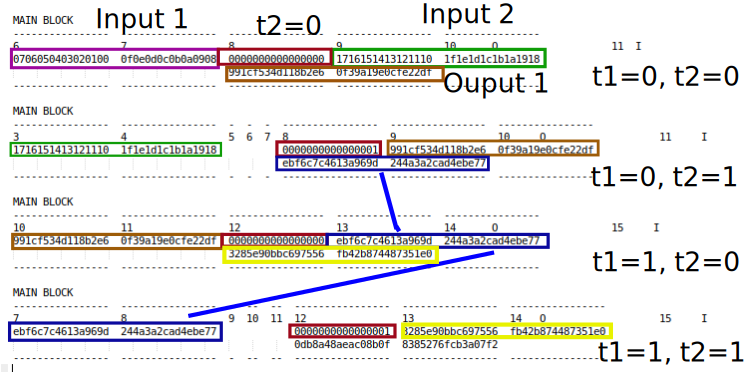
\includegraphics[width=0.9\textwidth]{./screenshots/p2_loop_b3_21f.v2.png}
  \caption{Données modifiées pour plusieurs itérations de \inlinetext{loop2_b3-21f}}
  \label{fig:p2_loop_b33_21f}
\end{figure}

Chaque \inlinetext{MAIN BLOCK} correspond à une itération.
La première ligne correspond aux entrées lues et la deuxième aux entrées de la stack modifiées par la boucle.
Les logs ont été tronqués mais au total 8 itérations de la boucle ont été réalisées avant la fin du programme.

On peut faire plusieurs observations à ce niveau:
\begin{itemize}
  \item L'outer loop (loop1) fait 4 itérations et loop2 fait un \inlinepython{for range(2)} (le compteur fait 0-1, 0-1...)
  \item Le boucle prend deux entrées (1 entrée = 2 qword) hors compteur et produit 2 qw.
  \item $output_n = input2_{n+1} = input1_{n+2}$
\end{itemize}


Le pseudocode des deux premières boucles ressemblent alors à:
\begin{minted}[breaklines]{python}
def loop1(flag_low, flag_high):
  L, H = flag_low, flag_high
  for counter1 in range(4): # loop1
    L, H = H, G(L, H, 0) # loop2 iter 0
    L, H = H, G(L, H, 1) # loop2 iter 1
  return L, H
\end{minted}

À partir de là, ca sent le cipher vraiment similaire à un feistel network.
\begin{figure}[H]
\centering
\includegraphics[width=0.9\textwidth]{./screenshots/800px-Feistel_cipher_diagram_en.svg.png}
  \caption{Feistel network}
  \label{fig:feistel}
\end{figure}

On continue l'étude du programme en regardant la boucle suivante: \inlinetext{loop3_154-210}.

\begin{minted}[breaklines]{bash}
$ python main.py --actions=compute_stats --dwarf-file=./dwarf.state.ir2.pickle  --run-ir --fixed-sp  --tgt-spec=0x154,0x210,None   --tgt-repeat=66 > ./logs/trace-154-210.out
\end{minted}



\begin{figure}[H]
\centering
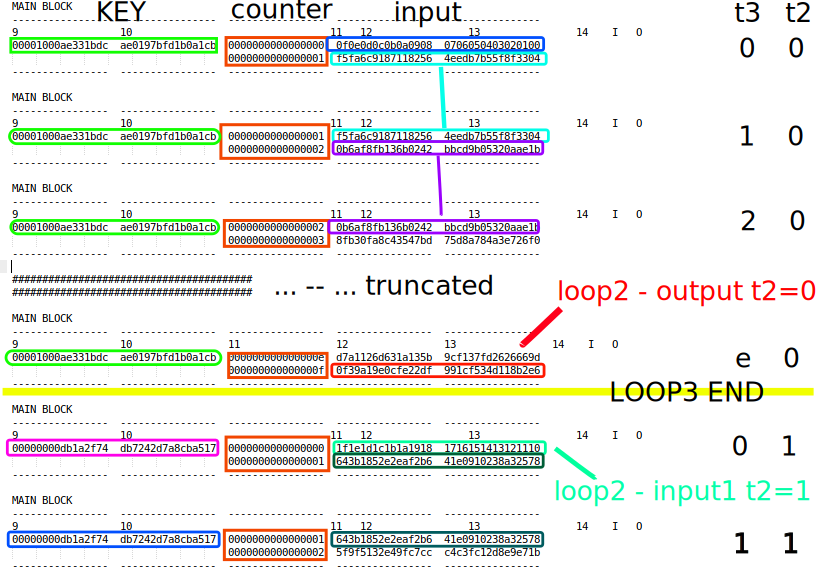
\includegraphics[width=0.9\textwidth]{./screenshots/p2_154-210.png}
  \caption{Données modifiées pour plusieurs itérations de \inlinetext{loop3_154-210}}
  \label{fig:p2_loop_154_210}
\end{figure}

Les données colorées sur la figure \ref{fig:p2_loop_154_210} sont assez explicites. On peut facilement en déduire le fonctionnement haut-niveau de l'algo:
\begin{minted}[breaklines]{python}
def loop3(key, input):
  x = input
  for i in range(15):
    x = F(key, i, x)
  return x

def G(L, H):
  key = KDF(L,H)
  return swap_qword(loop3(key, swap_qword(L)))
\end{minted}

Pas besoin de continuer plus loin, on a assez d'informations pour inférer le fonctionnement de l'algorithme (même si les outils développés permettent de vérifier rapidement ces inférences) ainsi que pour retrouver le flag.

En effet, on a aussi pu remarquer dans les instructions dwarf vers la fin du programme:
\begin{minted}[breaklines]{text}
002d 0e DW_OP_const8u  0x658302a68e8e1c24
0036 27 DW_OP_xor 
0037 16 DW_OP_swap 
0038 0e DW_OP_const8u  0xdc7564f1612e5347
0041 27 DW_OP_xor 
0042 22 DW_OP_plus 
0043 16 DW_OP_swap 
0044 0e DW_OP_const8u  0xd9c69b74a86ec613
004d 27 DW_OP_xor 
004e 22 DW_OP_plus 
004f 16 DW_OP_swap 
0050 0e DW_OP_const8u  0x65850b36e76aaed5
...
jump to win or fail
\end{minted}

Des XOR de 4 qwords...

On en déduit:
\begin{itemize}
  \item Ca ressemble à un algo d'encryption + comparaison de 32 octets pour un flag de 32 octets => la bijection sera facilement réversible car les 32 octets rendent le bruteforce impossible
  \item  => KDF(L,H) = KDF(H)
  \item  => F(k, i, x)  => $F_{k,i}(x)$ est inversible
\end{itemize}


Inverser l'algorithme donne quelque chose du genre:
\begin{minted}[breaklines]{python}
def invert_loop1(L, H):
  for i in range(4):
    L, H = invert_G(H, L), L
    L, H = invert_G(H, L), L

  flag_low, flag_high = L, H
  return flag_low, flag_high

def invert_G(Lcrypt, H):
  key = KDF(H)
  return swap_qword(invert_loop3(key, swap_qword(Lcrypt)))

def invert_loop3(key, input_crypt):
  x = input_crypt
  for i in reversed(range(15)):
    x = invert_F(key, i, x)
  return x
\end{minted}


Cool, on a une vue générale de l'algo pour retrouver le flag mais il manque les briques élémentaires: \inlinepython{KDF} et \inlinepython{invert_F}.
Et c'est là que tout ce qui a été développé jusque-là paie (l'opération générale reste probablement déficitaire :) ).

\begin{itemize}
\item \inlinepython{KDF} peut être calculée en black box par les instructions dwarf.

\item La fonction \inlinepython{F} est convertie en ELF en compilant le programme \inlinebash{0x154 - 0x20f} avec llvmpy.
angr rentre enfin en jeu pour inverser F.
\end{itemize}
À titre indicatif, le code qui utilise angr est le suivant:

\begin{minted}[breaklines]{python}
class AngrSolver:
  def __init__(self, infile):

    proj = angr.Project(infile)
    self.good_func = proj.loader.find_symbol('good')
    self.bad_func = proj.loader.find_symbol('bad')
    self.proj = proj


  def solve1(self, fixed_input, n_find, fixed_output):
    # fixed_input: key + counter
    # n_find: number of qword we need to find
    # x in invert_loop3

    b1 = StreamRW(bytearray([0]*len(fixed_input)*8), arch=Arch.x86_64)
    b1.write_nu64(0, fixed_input)
    b2 = StreamRW(bytearray([0]*len(fixed_output)*8), arch=Arch.x86_64)
    b2.write_nu64(0, fixed_output)

    inx =  claripy.BVV(bytes(b1.buf))
    input_var =  claripy.BVS('unknown', 64 * n_find)

    # l'ELF permet de prendre en entrée l'état de la stack initial
    # ainsi que l'état final attendu.
    # Le code est ensuite exécuté.
    # La fonction good() est appelée si le résultat est le bon, sinon bad()
    data = claripy.Concat(claripy.BVV(bytes(b2.buf + b1.buf)), input_var)


    initial_state = self.proj.factory.entry_state(args=['abc', data])
    sm = self.proj.factory.simulation_manager(initial_state)
    sm.explore(find=self.good_func.rebased_addr, avoid=self.bad_func.rebased_addr)
    found = sm.found[0]
    buf = found.solver.eval(input_var, cast_to=bytes)
    buf = StreamRW(buf, arch=Arch.x86_64)
    res = buf.read_nu64(0, n_find)
    return res

\end{minted}

Bon, ça prend quand même pas mal de temps, y'a $15 \times 2 \times4 = 120$ appels fait à angr. De souvenir y'a au moins une heure de calculs mais ca vaut bien une esquive magique du reverse de la fonction F.


Le flag tombe alors:
\begin{minted}[breaklines, escapeinside=||]{text}
|\textcolor{green}{\detokenize{SSTIC{Dw4rf_VM_1s_co0l_isn_t_It}}}|
\end{minted}

\pagebreak
\section{Niveau 3 - SecureOS}

En validant le dernier flag, on nous demande de reboot:
\begin{minted}[breaklines, escapeinside=||]{text}
# /root/tools/add_key.py SSTIC{Dw4rf_VM_1s_co0l_isn_t_It}
[+] Key with key_id 00000003 ok
[+] Key added into keystore
[+] Envoyez le flag SSTIC{Dw4rf_VM_1s_co0l_isn_t_It}} à l'adresse challenge2019@sstic.org pour valider votre avancée
[+] Container /root/safe_02/.encrypted decrypted to /root/safe_02/decrypted_file
[w] |\textcolor{red}{You must reboot in order to decrypt Secure OS}|
\end{minted}


\subsection{Binaire userspace}
On va avoir droit à un programme tournant en hyperviseur ou dessous. En se renseignant sur le net, on tombe sur:
\begin{figure}[H]
\centering
\includegraphics[width=0.9\textwidth]{./screenshots/map_processor_modes_to_aarch32.png}
  \caption{Mode d'un processeur arm}
  \label{fig:p3_processor_modes}
\end{figure}
Y'a des chances que ça tourne dans le Secure Monitor (EL3).


C'est bien beau de supposer mais pour en avoir le coeur net, on peut faire un \inlinebash{strace} du programme pour glaner rapidement des informations:
\begin{minted}[breaklines]{strace}
07:36:19 execve("/root/safe_02/decrypted_file", ["/root/safe_02/decrypted_file", "aaaaaaaaaaaaaaaaaaaaaaaaaaaaaaaa"...], 0xffffdc318fc0 /* 10 vars */) = 0
07:36:19 brk(NULL)                      = 0x20a8d000
07:36:19 brk(0x20a8df80)                = 0x20a8df80
07:36:19 uname({sysname="Linux", nodename="sstic", ...}) = 0
07:36:19 readlinkat(AT_FDCWD, "/proc/self/exe", "/root/safe_02/decrypted_file", 4096) = 28
07:36:19 brk(0x20aaef80)                = 0x20aaef80
07:36:19 brk(0x20aaf000)                = 0x20aaf000
07:36:19 openat(AT_FDCWD, "/dev/sstic", O_RDONLY) = 3
07:36:19 ioctl(3, SEV_ISSUE_CMD, 0xffffd88349f8) = 0
07:36:19 ioctl(3, _IOC(_IOC_READ|_IOC_WRITE, 0x53, 0x1, 0x10), 0xffffd88349f8) = 0
07:36:19 ioctl(3, _IOC(_IOC_READ|_IOC_WRITE, 0x53, 0x2, 0x10), 0) = 0
07:36:19 ioctl(3, SNDRV_SEQ_IOCTL_RUNNING_MODE, 0) = 0
07:36:19 ioctl(3, _IOC(_IOC_READ|_IOC_WRITE, 0x53, 0x2, 0x10), 0) = 0
07:36:19 ioctl(3, SNDRV_SEQ_IOCTL_RUNNING_MODE, 0) = 0
07:36:19 ioctl(3, _IOC(_IOC_READ|_IOC_WRITE, 0x53, 0x2, 0x10), 0) = 0
....
07:36:41 ioctl(3, _IOC(_IOC_READ|_IOC_WRITE, 0x53, 0x2, 0x10), 0) = 0
07:36:41 ioctl(3, SNDRV_SEQ_IOCTL_RUNNING_MODE, 0) = 0
07:36:41 ioctl(3, _IOC(_IOC_READ|_IOC_WRITE, 0x53, 0x2, 0x10), 0) = 0
07:36:41 ioctl(3, SNDRV_SEQ_IOCTL_RUNNING_MODE, 0) = 0
07:36:41 ioctl(3, _IOC(_IOC_READ|_IOC_WRITE, 0x53, 0x2, 0x10), 0) = 0
07:36:41 ioctl(3, SNDRV_SEQ_IOCTL_RUNNING_MODE, 0) = 65537
07:36:41 fstat(1, {st_mode=S_IFCHR|0600, st_rdev=makedev(5, 1), ...}) = 0
07:36:41 ioctl(1, TCGETS, {B115200 opost isig icanon echo ...}) = 0
07:36:41 write(1, "Loose\n", 6)         = 6
07:36:41 exit_group(0)                  = ?
07:36:41 +++ exited with 0 +++
\end{minted}

\filename{/dev/sstic} et du \inlinec{ioctl}, pas étonnant que ça passe par le kernel pour aller dialoguer avec le Secure Monitor.
On observe tout de suite qu'il y a 4 types d'ioctl: 2 d'initialisations et 2 de polling. En jetant rapidement un oeil dans ida, cela se confirme.
Un des ioctl de polling retourne 0 tant que le résultat n'est pas prêt puis un résultat non-zéro.
\begin{minted}[breaklines]{strace}
07:36:41 ioctl(3, SNDRV_SEQ_IOCTL_RUNNING_MODE, 0) = 65537 # 0x10001
\end{minted}


En étudiant un peu plus le binaire userspace dans ida, on arrive sans trop de difficulté à un algo reflété par le pseudocode suivant:

\begin{minted}[breaklines]{c}
ioctl INIT (0x044DBD8 , 0x101010 ) // secret_data, secret_data_len
ioctl LOAD_DATA (bin_argv[1], 0x20) //sending flag
while (true){
  ioctl(QQ) // nop?
  int res = ioctl(QUERY);
  reslow = res & 0x0000ffff;
  reshigh = res & 0xffff0000;
  if (reslow==1){
    if (reshigh==0) win();
    else loose();
  } else {
    if (reslow == 0xffff) failure();
  }
}
\end{minted}

On cherche ensuite à identifier le binaire du module kernel.
\subsection{Module kernel}
\begin{tcolorbox}
\begin{lstlisting}[escapechar=~]
$ lsmod
Module                  Size  Used by    Not tainted
sstic                  16384  0
$ find / -name "*.ko"
/lib/sstic.ko
$ strings /lib/sstic.ko
9u(r
Linux
alias=platform:sstic
license=GPL
description=~\textcolor{red}{Driver for SSTIC Challenge : Communication between normal world and Secure world}~
author=David BERARD <contact@davidberard.fr>
depends=
intree=Y
name=sstic
\end{lstlisting}
\end{tcolorbox}

Parfait, on a trouvé le module: \inlinebash{/lib/sstic.ko}. En l'ouvrant dans ida, on trouve sans problème la fonction \inlinec{sstic_ioctl}, visible en figure \ref{fig:p3_kern_module_ioctl}.

\begin{figure}[H]
\centering
\includegraphics[width=0.9\textwidth]{./screenshots/p3_kern_module_ioctl.png}
  \caption{Fonction sstic\_ioctl du module noyau /lib/sstic.ko}
  \label{fig:p3_kern_module_ioctl}
\end{figure}

Encore une fonction tentaculaire. On s'attend bien évidemment à trouver du \inlinec{kmalloc} et du \inlinec{copy_from_user}. Effectuer un tracing manuel est faisable mais assez pénible. Il est temps de sortir le débuggeur.
QEMU permet de lancer un \inlinebash{gdbserver} que l'on peut ensuite connecter avec \inlinebash{aarch64-linux-gnu-gdb}. Y'a pleins de tutos pour le net, mais en quelques mots:
\begin{minted}[breaklines]{bash}
  Terminal 1                                                  Terminal 2
$ ${QEMU_COMMAND} -monitor pty
$ minicom -D /dev/pts/${PTS_DU_QEMU}
gdbserver
                                                        $ aarch64-linux-gnu-gdb
                                                        target remote :1234
                                                        {session gdb normale...}
\end{minted}

Il est possible de mettre des breakpoints sur les fonctions du module kernel (comme \inlinec{sstic_ioctl}) en récupérant le \inlinebash{/proc/kallsyms} du téléphone:

\begin{tcolorbox}
\begin{lstlisting}[escapechar=@]
$ cat /proc/kallsyms | grep sstic
...
  ffff000008590000 t $x   [sstic]
  @\textcolor{red}{ffff000008590000 t sstic\_open   [sstic]}@
  @\textcolor{red}{ffff000008590020 t sstic\_release        [sstic]}@
  @\textcolor{red}{ffff000008590038 t sstic\_ioctl  [sstic]}@
  ffff000008590604 t $x   [sstic]
  ffff000008590604 t sstic_exit   [sstic]
  ffff000008592000 d $d   [sstic]
  ffff000008592000 d pugs_fops    [sstic]
  ...
\end{lstlisting}
\end{tcolorbox}


Avec le remote gdb, on peut alors tracer \inlinec{sstic_ioctl} pour les différents types d'ioctl.
Comme attendu, le module noyau fait quasi-exclusivement du proxying vers les rings inférieurs avec l'instruction \inlinebash{smc}.

\subsection{Améliorer le workflow de test}
Tout d'abord, y'a un besoin important de toolup pour améliorer le workflow de test, qui requiert:
\begin{itemize}
  \item Lancer qemu (stoppé au démarrage ou non)
  \item Activer gdbserver
  \item Connecter un remote gdb
  \item Lancer le programme par ssh
  \item Piloter le trace-event de qemu
  \item Piloter le débuggeur
\end{itemize}

Réaliser tout ça manuellement n'est pas tenable pour expérimenter rapidement. Après le développement d'un tel outil, le workflow pouvait s'exprimer par:

\begin{minted}[breaklines]{python}
gx = SyncWrapper(self.gdb, self.el) # représente le débugger (api python de gdb)
                                    # proxy les appels vers le mainthread
qx = get_qemu(self.ctx.qemu_pts) # qemu
sx = get_ssh() #ssh

Z.time.sleep(0.2)
qx('stop') # stop qemu, synchrone
qx('trace-file off')

qx('gdbserver') # active gdbserver
gx.do_execute('target remote :1234') # connect gdb
print('Target connected')

sx.run(self.ctx.prog_cmd) # lance le programme avec le bon flag, async nowait
gx.run_to(init_done_km) # execute jusqu'au pc demandé
gx.do_execute('gef config context.enable False')
\end{minted}

A partir de là, je fus bloqué assez longtemps avant de trouver le code réalisant la vérification du flag (objectif atteint je suppose pour le problème setter).

\subsection{Hall of fail}

Ce blocage vient en grande partie de l'échec des \og hardware \fg breakpoints sur les accès mémoires dans qemu.
En effet, ceux-ci ne fonctionnent pas pour certaines instructions récentes (ARMv8.2), utilisées par notre secure monitor. Aussi, ces instructions ne sont pas supportées dans ma version d'ida donc le scan de fonctions  s'est bien raté. La confusion fut efficace.
Mais ces faits n'étaient pas connus à l'époque. De plus, en googlant à postériori y'a peut-être des repos sur le net qui proposent de tweaker ida pour supporter ces nouvelles instructions.


En faisant tourner le programme, c'est comme si le flag ou les données initiales envoyées par le programme n'étaient jamais utilisées.


J'ai donc eu la chance de creuser dans de mauvaises directions.

\subsection {Trouver des patternes d'accès mémoires et instructions via le event qemu}


Qemu possède des fonctionnalités pour tracer des évènements. On peut notamment récupérer des logs sur les accès mémoires ainsi que sur l'enchainement des \inlinec{struct TranslationBlock} exécutés (~= ensemble consécutif d'instructions).

Pour cela il suffit de rentrer dans le monitor qemu les commandes suivantes (après avoir recompilé qemu et le support des traces, notamment pour la commande trace-file):
\begin{minted}[breaklines]{text}
trace-event guest_mem_before_exec on
trace-event exec_tb on
trace-file on
cont # exécution de la partie qui nous intéresse à tracer
...
trace-file off
trace-event guest_mem_before_exec off
trace-event exec_tb off
\end{minted}

Une fois la trace obtenue, on peut la convertir en format texte:
\begin{minted}{bash}
${g_qemu_path}/scripts/simpletrace.py ${g_qemu_path}/trace-events-all  ${trace_file} > ${temp_file}
\end{minted}

À noter que j'ai patché le format de la trace de \inlinetext{guest_mem_before_exec}, sans grande importance

\begin{minted}{text}
guest_mem_before_exec 0.198 pid=23400 __cpu=0xe0492c8 vaddr=0xe0492c9 info=0xff
exec_tb 13.153 pid=23400 tb=0x7f637c113f40 pc=0xe0355e4
guest_mem_before_exec 0.312 pid=23400 __cpu=0xe04a59b vaddr=0xe04a59c info=0xff
guest_mem_before_exec 1.446 pid=23400 __cpu=0xe038748 vaddr=0xe038749 info=0xff
exec_tb 13.431 pid=23400 tb=0x7f637c114180 pc=0xe0355f8
guest_mem_before_exec 0.322 pid=23400 __cpu=0xe0492e0 vaddr=0xe0492e1 info=0xff
guest_mem_before_exec 0.250 pid=23400 __cpu=0xe0492e8 vaddr=0xe0492e9 info=0xff
guest_mem_before_exec 0.264 pid=23400 __cpu=0xe0492f0 vaddr=0xe0492f1 info=0xff
exec_tb 8.385 pid=23400 tb=0x7f637c114440 pc=0xe032014
exec_tb 3.957 pid=23400 tb=0x7f637c1145c0 pc=0xe032024
exec_tb 50.307 pid=23400 tb=0x7f637c1146c0 pc=0xe031034
guest_mem_before_exec 0.658 pid=23400 __cpu=0xe0492d0 vaddr=0xe0492d1 info=0xff
guest_mem_before_exec 3.386 pid=23400 __cpu=0xe03af70 vaddr=0xe03af71 info=0xff
\end{minted}


Une telle trace peut être convertie pour la visualiser avec TraceGraph de SideChannel-Marvels (\url{https://github.com/SideChannelMarvels/Tracer/tree/master/TraceGraph}).
La conversion de la trace textuelle au format attendu dans des tables sqlite3 est anecdotique et réalisée en python.

On obtient alors:

\begin{figure}[H]
  \centering
  \vertfig[TraceGraph partie 1]{
    %\includegraphics[width=\textwidth]{../virtual_phone/safe_01/graphs/{t_tx1_05.dot}.ps}
    %\includegraphics[width=\textwidth]{../virtual_phone/safe_01/graphs/{t_tx1_05.dot}.ps}
    \includegraphics[width=\textwidth]{./screenshots/p3_tracegraph_low.png}
  }
  \hfill
  \vertfig[TraceGraph partie 2]{
    %\includegraphics[width=\textwidth]{../virtual_phone/safe_01/graphs/{t_tx1_05.dot}.ps}
    %\includegraphics[width=\textwidth]{../virtual_phone/safe_01/graphs/{t_tx1_05.dot}.ps}
    \includegraphics[width=\textwidth]{./screenshots/p3_tracegraph_high.png}
  }
  \caption{Accès mémoire / instructions lors de l'exécution d'une partie du programme}
  \label{fig:p3_tracegraph}
\end{figure}

Sur ce graphe, on peut observer que la partie des données centrale (\inlinec{init_data}) est stockée en 0xe053000 - 0xe15410) avec le buffer fourni par le binaire mais n'est pas utilisée après cela.

Pour vérifier ce comportement inattendu, j'ai modifié le contenu de ce buffer avant chargement.
Le comportement du programme fut totalement différent (un message d'erreur autre il me semble), en contradiction directe avec l'expérience précédente.


Pas cool de pas avoir de trace d'évènement mémoire. Passons à la prochaine tentative.


\subsubsection {Essayer de fixer qemu}
La machine virt de qemu possède une ram normale et une secure ram. 
Peut-être des mappings différents font que les breakpoints ne sont pas déclenchés.

Il est indiqué dans l'énoncé du chall qu'il ne fonctionne qu'avec une version précise et récente de qemu. Il est donc imaginable qu'il y ait des problèmes dans cette version au niveau des breakpoints.
Des suppositions à moitié stupide ont donc été faites dans un état de compréhension très limité de qemu et de l'arm hors userspace.


\begin{itemize}
\item Patcher qemu et appeler \inlinec{hw_breakpoint_update} à chaque exception/interrupt pour que le changement
\item Désactiver le secure ram attribut
\item Jouer avec les \inlinec{struct AddressSpace}
\end{itemize}

Tout ces essaies échouèrent.

\subsubsection {Reverse du bootloader}
Un peu à court d'idée à ce niveau, j'ai eu la mauvaise idée de regarder ce que faisait le bootloader.
Je me suis alors trouvé à reverse l'arm trusted firmware ( \url{https://github.com/ARM-software/arm-trusted-firmware}), et identifier les \inlinec{bl31_main} jusqu'aux \inlinec{oem_smc_handler} et \inlinec{tspd_std_smc_handler}.


Refaire les étapes mentionnées dans le firmware-design (\url{https://chromium.googlesource.com/external/github.com/ARM-software/arm-trusted-firmware/+/v0.4-rc1/docs/firmware-design.md}) c'est cool mais pas très utile.
Bref une période très sombre de ce chall.


\subsection{Découverte de SM4}

En traçant l'ioctl qui effectue le chargement du flag on tombe sur des instructions sm4key et sm4e dans la fonction en 0xE200E84 (que je dénoterai \inlinec{secure_mem_rw}). J'ai mis du temps à détecter ça car ni ida ni ma version de capstone ne connaissaient ces instructions récentes, qui n'apparaissaient donc pas dans ma trace (silencieusement).
Ces instructions sont relatives à l'encryption/décryption (qui sont équivalentes) avec le cipher chinois SM4 (\url{https://en.wikipedia.org/wiki/SM4_(cipher)}). Elles opèrent sur 16 octets.

On y trouve à côté des expressions vectorisées (\inlinec{ld1, st1, rev32}) qui ne trigger pas les breakpoints mémoire qemu. Voilà nos coupables! \\ 


Aussi, cette fonction n'est jamais appelée directement:
Lorsqu'une instruction (load ou store) essaie d'accéder à de la mémoire située dans le range (0 - 0x10040),  une exception est levée et le handler \inlinec{secure_mem_rw} est appelé.
Ce handler va alors décrypter une partie de la mémoire dans le range (0xE053000, 0xe153040) et retourner ou modifier le bon dword puis ré-encrypter la mémoire.
Des mots de 16 octets sont considérés (intrinsèque au cipher SM4). Des précautions doivent donc être prise pour les dwords s'étalant sur la frontière de deux mots sm4.


Le pseudocode ci-dessous exprime l'idée générale des accès mémoires:

\begin{minted}[breaklines]{python}
sm4_mem_base = 0xe053000
# la clé sm4 est une fonction d'un terme fixe et de l'adresse -> elle est différente pour chaque bucket

def handler_secure_mem_rw(addr, is_read, content=None):

  addr1 = addr & ~0xf # alignement sur 16 octets
  addr2 = addr1 + 0x10
  buf = sm4_read(addr1) + sm4_read(addr2) # 16 bytes + 16 bytes -> 32bytes
  offset= addr&0xf:

  if is_read:
    return buf[offset:offset+4]
  else:
    buf[offset:offset+4] = content
    sm4_write(addr1, buf[:0x10])
    sm4_write(addr2, buf[0x10:])
\end{minted}


Juste placer des taps sur ces accès mémoires ne permet pas de comprendre le fonctionnement de l'algo car bien que le flag y soit stocké puis lu au début, très peu d'accès en écriture y sont fait.

\subsection{Dispatcher du secureos}

En cherchant les endroits qui trigger ces accès mémoires, on trouve une fonction intéressante du secureos en 0xE2005A4, dénommée \inlinec{dispatch_func}.
Cette fonction lit des informations de la mémoire sm4 et à partir de là décide d'exécuter telle ou telle branche.
Bon, à partir de là on a plus ou moins trouver le dispatcher de notre VM.
\begin{figure}[H]
\centering
\includegraphics[width=0.8\textwidth]{./screenshots/p3_secureos_dispatch_func.png}
  \caption{Fonction de dispatch du secureos en 0xE2005A4, dénommée \inlinec{dispatch_func}}
  \label{fig:p3_dispatcher}
\end{figure}

Comme on peut le voir sur le figure \ref{fig:p3_dispatcher}, cette fonction est assez chelou, y'a pleins de blocs de degré entrant ou sortant zéro.
Il doit y avoir plusieurs raisons pour cela:
\begin{itemize}
  \item Certaines instructions d'ARMv8-a sont pas supportées par ida (fcmla notamment)
  \item des blocs appellent une fonction faisant un ERET
  \item Des instructions de la VM sont dispatchées avec un beau switch qui perturbe ida (br x0 en 0x0E2007E8, voir fig \ref{fig:p3_dispatch_br})
\end{itemize}

\begin{figure}[H]
\centering
\includegraphics[width=0.8\textwidth]{./screenshots/p3_dispatch_br.png}
  \caption{Dispatch par un switch like}
  \label{fig:p3_dispatch_br}
\end{figure}

On trouve dans le dispatcher des ERET, SMC (secure monitor call) et des accès à la mémoire sm4: y'a encore du boulot.


\subsection{Dispatcher du el2}

En traçant les SMC, ils atterrissent finalement en 0xE032014 (\inlinec{oem_smc_handler}).

\begin{figure}[H]
\centering
\includegraphics[width=0.8\textwidth]{./screenshots/p3_oem_svc_handler.png}
  \caption{Fonction \inlinec{oem_smc_handler} en 0xE0311BC}
  \label{fig:p3_oem_smc_handler}
\end{figure}

La fonction présentée par ida est visible en figure \ref{fig:p3_oem_smc_handler} et plus particulièrement en E0311BC


J'étais déjà passé par cette fonction auparavant sans que rien ne saute aux yeux.
En suivant la trace dans cette fonction, on trouve un certain point de passage familier, un bon switch:
\begin{minted}{gas}
ADR             X1, loc_E0311C0
ADD             X0, X1, W0,SXTH#2
br x0
\end{minted}

Dans ida ça ressemble à:

\begin{figure}[H]
\centering
\includegraphics[width=0.8\textwidth]{./screenshots/p3_oem_smc_dispatch.png}
  \caption{Switch dispatch dans \inlinec{oem_smc_handler}}
  \label{fig:p3_oem_smc_dispatch}
\end{figure}

Hum, pourquoi la partie du bas est en rouge? Une fonction se termine rarement avec une branch inconditionnelle.
Eh oui, on retrouve plus bas encore des instructions que mon ida ne connait pas.
Cette fois-ci on trouve des instructions \inlinec{aese, aesd, fcadd, dup, ...}.
Un bref descriptif de ces instructions:

\begin{itemize}
    \item aese, aesd: effectue un round d'aes
    \item fcadd, dup, ld1, st1: instructions arm vectorielles sur des registres spéciaux (v0, v1, v2...): addition sur complex, chargement depuis registre normal, load et store
\end{itemize}
Hum, ca explique pourquoi mes tests d'exécution différentielle n'ont pas fonctionné, je ne loggais pas ces registres vectoriels.



Deux dispatchers, ca fait quand même beaucoup.
En plaçant des taps sur les 2 switchs, on peut connaître comment sont appelées les opérations. Une fois de plus on utilise TraceGraph pour représenter les données

\begin{figure}[H]
\centering
\includegraphics[width=0.8\textwidth]{./screenshots/p3_vmops_2.png}
  \caption{Visualisation des opérations de la VM dans TraceGraph}
  \label{fig:p3_vmops}
\end{figure}

Sur la figure \ref{fig:p3_vmops}, plusieurs phases peuvent être observées:
\begin{itemize}
    \item une phase principale qui consiste en 4 itérations
    \item une phase de vérification
\end{itemize}




\subsection{VM ops de l'EL2}

Le dispatcher du secureos \inlinec{dispatch_func} est quand même bien compliqué avec ses exceptions SM4, ses ERET et SMC qui vont appeler le dispatcher de l'EL2 \inlinec{oem_smc_handler}.

Je décide donc de me concentrer sur les opérations faites par l'EL2.
Toutes ces opérations ont un pattern similaire:
\begin{minted}[breaklines]{text}
a = ld1 *(0xe04a5d8 +base)
a = aese a, flag_substr
a = eor a, flag_substr

some vector operation on a

aesd a, flag_substr
eor a, flag_substr
st1 a, *(0xe04a5d8 +base)
\end{minted}

En somme, ces opérations font: décryption des données, opération sur ces données, encryption du résultat.
On observe que \inlinetext{base} ne prend pas plus de 16 valeurs. Les données encryptées par AES sont au nombre de 16, là où celles par SM4 s'étalaient sur 0x100040 octets.

On peut ainsi penser la mémoire AES comme des registres et la mémoire SM4 comme une RAM.


Avec un peu de travail manuel pour chacune de ces opérations et avec du single stepping automatisé qui log les registres modifiés à chaque instruction, il est assez aisé de reverse toutes les opérations effectuées par nos VM ops.
Ces opérations sont résumées dans le tableau \ref{table:el2_funcs}.


\begin{table}[h!]
  \centering
\begin{tabular}{|c|c|l|}
  \hline
  Function & Addr & Opérations \\
  \hline
  FUNCA& 000000000e0311c0 & return reg[x19] \\
  \hline
  FUNCB& 000000000e031234 & reg[x19] = w2 \\
  \hline
  FUNCC& 000000000e03132c & reg[x19] += reg[x22]; pc += 3; \\
  \hline
  FUNCD& 000000000e031518 & reg[x19] -= reg[x22]; pc += 3; \\
  \hline
  FUNCE &000000000e031608 & reg[x19] $\wedge$= reg[x22]; pc += 3; \\
  \hline
  FUNCF &000000000e0317f4 & reg[x19] --; \\ 
  \hline
  FUNCG &000000000e031b58 & reg[x19] += x22; pc += 3; \\
  \hline
  FUNCH &000000000e031bf4 & reg[x19] -= x22; pc += 3; \\
  \hline
  FUNCI &000000000e031df0 & reg[x19] \&= x22; pc += 3; \\
  \hline
  FUNCJ &000000000e031e9c & pc = x22;\\
  \hline
\end{tabular}
  \caption{VM ops du dispatcher EL2}
\label{table:el2_funcs}
\end{table}

La découverte du "pc" ne fut faite qu'en exécutant le programme avec des taps placés sur chacune de ces opérations, le dispatcher SecureOS ainsi que sur les lectures et écriture dans la mémoire SM4.


\subsection{\:Extraction de la mémoire SM4}

La zone de mémoire encryptée SM4 est utilisées par l'algo et devra donc être décryptée si on souhaite émuler le programme en python par exemple.
Dans ce but, j'ai utilisé le code de qemu pour les instructions SM4*, disponible dans le fichier \inlinebash{qemu/target/arm/crypto_helper.c}.
Á partir de ce fichier on peut extraire les fonctions liées à sm4 et patcher légèrement pour créer des bindings python avec SWIG afin de rendre disponible en python les instructions sm4.

Effectuer le bon decryptage après ça (usage des bonnes clés, gestion des rev32 (reverse des octets)) peut facilement être obtenu avec une trace.
Le résultat en python est alors:
\begin{minted}[breaklines]{python}
  def get(self, q):
    kq = q & ~0xf
    if self.raw_data: # fastpath une fois que tout a été décodé
      return self.raw_data[kq // 16]

    tgt = self.data[kq:kq + 0x10]

    u = Z.swig_unsafe.hack_ctf_sstic_2019_swig

    k = Z.struct.unpack('<IIII', self.k) # hardcoded key
    k = [x ^ kq for x in k] # key mixed with address
    ks = Z.struct.pack('<IIII', *k)
    kk = u.opa_crypto_sm4ekey(self.n, ks) # instruction sm4key

    #rev32
    tgt = b''.join([tgt[i:i + 4][::-1] for i in range(0, 16, 4)])

    kk = Z.struct.unpack('<IIII', kk)
    kk = Z.struct.pack('<IIII', *kk[::-1])
    res = u.opa_crypto_sm4e(tgt, kk) # instruction sm4e
    return res[::-1]
\end{minted}


P.S: effectuer le décryptage en scriptant le débuggeur c'est plus simple mais bien trop lent pour $2^{20}$ octets. Un code compilé arm et exécuté dans qemu aurait également pu marcher.


\subsection{\:Tentative de résolution 1 - échec}
À partir de là, je pensais être en mesure de reverse l'algo en utilisant les taps avec une exécution différentielle, en regardant comment les registres AES évoluent.

Pour obtenir deux traces, j'utilise la ligne de commande:
\begin{minted}{bash}
python solve.py --actions=test1 --qemu-pts=$CUR_PTS --verbosity=DEBUG   --from-shell  --output-dir=./trace/  --action2=do_tracing_op3 --trace-to=0 --runid=setup_to_192 --solve-ev --setup-begin
# va lancer /root/safe_02/decrypted_file 000102030405060708090a0b0c0d0e0f101112131415161718191a1b1c1d1e1f
python solve.py --actions=test1 --qemu-pts=$CUR_PTS --verbosity=DEBUG   --from-shell  --output-dir=./trace/  --action2=do_tracing_op3 --trace-to=0 --runid=setup_to_192-keya --key-a --solve-ev --setup-begin
# va lancer /root/safe_02/decrypted_file aaaaaaaaaaaaaaaaaaaaaaaaaaaaaaaaaaaaaaaaaaaaaaaaaaaaaaaaaaaaaaaa
\end{minted}


Les deux traces peuvent alors être diffées pour facilement voir où est traité le flag:
\begin{figure}[H]
\centering
\includegraphics[width=1.0\textwidth]{./screenshots/p3_diff_2.png}
  \caption{Extrait de diff entre deux exécutions}
  \label{fig:p3_diff_example}
\end{figure}

En essayant de reverse avec ce diff, j'ai pu obtenir un algo consistant d'une répétion de blocs du type:
\begin{minted}[breaklines]{python}
  cur = (cur & 0xff) << 8 | (v & 0xff)
  cur |= i << 16
  cur += 0x1000
  v = smem.access(cur)
\end{minted}


Le mixage des clés (flag) est fait du manière assez obscure et de nombreux xor avec des constantes viennent perturber ces itérations.

En parcourant le diff, j'ai aussi pu observer que certains octets de la clé n'impactaient pas les valeurs finales lors de la vérification.

Vraiment bizarre. J'avais déjà pu voir des différences de comportement lorsque la trace était effectuée avec des breakpoints ou avec des singlestep.
Anti-debug ou juste problème de qemu, je ne sais toujours pas. Toujours est-il que les adresses de retour des ERET diffèrent parfois entre le singlestep et les breakpoint ce qui cause un changement de comportement de l'algo. \\



En essayant de débugger cette différence, j'ai notamment pu découvrir que certains ERET du dispatcher SecureOS passent en Aarch32 (qui d'ailleurs perturbe gdb) où certaines opérations de l'algo sont réalisées (code très petit par contre).

Tous ces fonctionnements cachés avec en plus un observer effect, cpa cool.


\subsection{\:Obtenir une trace fiable}
Si qemu et ses breakpoints sont problématiques, y'a toujours moyen d'instrumenter qemu.
J'ai passé assez de temps à essayer de le modifier durant cette édition pour comprendre un peu comment il fonctionne.
Comme qemu compile le code qu'il exécute (les \inlinec{struct TranslationBlock}), il est nécessaire de modifier le compilateur de qemu (tcg - tiny code generator) pour placer des hooks. \\ 


Dans le fichier \inlinebash{target/arm/translate-a64.c}, la fonction
\begin{minted}{c}
static void disas_a64_insn(CPUARMState *env, DisasContext *s)
\end{minted}
peut être patchée avec, pour chaque fonction à tracer,  un code du style:

\begin{minted}{c}
if (pc == 0xe031234){ // FUNCB

    TCGv_i64 tcg_pc = tcg_const_i64(pc);
    TCGv_i64 x0 = read_cpu_reg(s, 19, true); // lecture x19
    TCGv_i64 x1 = read_cpu_reg(s, 22, true); // lecture x22
    TCGv_i64 x2 = read_cpu_reg(s, 2, true); // lecture x2
    TCGv_i64 x3 = read_cpu_reg(s, 23, true); // lecture x23

    F5_Func *genfn;
    genfn = gen_helper_f5_func;
    genfn(tcg_pc, x0, x1, x2, x3); // call external function with pc + regs
    tcg_temp_free_i64(tcg_pc);
    tcg_temp_free_i64(x0);
    tcg_temp_free_i64(x1);
    tcg_temp_free_i64(x2);
    tcg_temp_free_i64(x3);
}
\end{minted}

L'helper est défini par:
\begin{minted}{c}
void HELPER(f5_func)(uint64_t a, uint64_t b, uint64_t c, uint64_t d, uint64_t e)
{
  fprintf(opa_f, "%lx,%lx,%lx,%lx,%lx\n", a, b, c, d, e);
  fflush(opa_f);
}
\end{minted}

Ce code va logger certains registres à certains pc pour nous permettrent de connaître les paramètres d'appel de toutes les VM ops de l'EL2.
On recompile qemu et quand on relance, on obtient une trace avec les valeurs du pc et de 4 autres registres aux points sélectionnés avec en tout 43k opérations.


Pour illustrer, cela nous donne des entrées du type:
\begin{minted}{text}
...
e0311c0,a,0,0,0
e200e84,6baee,0,0,e207240
e031234,5,3b7a2f70,3b7a2f70,0
e0311c0,f,0,0,0
e031234,f,a5,a5,0
e0311c0,f,0,0,0
e200e84,a5,0,0,e207280
e031df0,5,ff,ff,0
e0311c0,f,0,0,0
e200e84,a8,0,0,e207280
e0311c0,7,0,0,0
\end{minted}

qui peuvent être ensuite reconvertie en python pour être plus explicite:
\begin{minted}{python}
{'name': 'FUNCA', 'args': [10, 0, 0, 0]}
{'name': 'FUNC_RW_RAM', 'args': [441070, 0, 0, 237007424]}
{'name': 'FUNCB', 'args': [5, 997863280, 997863280, 0]}
{'name': 'FUNCA', 'args': [15, 0, 0, 0]}
{'name': 'FUNCB', 'args': [15, 165, 165, 0]}
{'name': 'FUNCA', 'args': [15, 0, 0, 0]}
{'name': 'FUNC_RW_RAM', 'args': [165, 0, 0, 237007488]}
{'name': 'FUNCI', 'args': [5, 255, 255, 0]}
{'name': 'FUNCA', 'args': [15, 0, 0, 0]}
{'name': 'FUNC_RW_RAM', 'args': [168, 0, 0, 237007488]}
{'name': 'FUNCA', 'args': [7, 0, 0, 0]}
\end{minted}

\subsection{\:Schéma global du système}


Avec toutes les informations glanées, on peut dresser un schéma global du système, visible en figure \ref{fig:p3_diag}.
\begin{figure}[H]
\centering
\includegraphics[width=0.8\textwidth]{./screenshots/diag.png}
  \caption{Diagramme global du système}
  \label{fig:p3_diag}
\end{figure}


\subsection{\:Automatiser le reversing}

La tentative précédente, perturbée par l'observer effect, m'a refroidi sur le reverse manuel. On va donc essayer d'automatiser un petit peu plus.


Avec le patch précédent, on récupère une trace d'exécution pour différents flags:
\begin{minted}{bash}
/root/safe_02/decrypted_file 000102030405060708090a0b0c0d0e0f101112131415161718191a1b1c1d1e1f
/root/safe_02/decrypted_file aaaaaaaaaaaaaaaaaaaaaaaaaaaaaaaaaaaaaaaaaaaaaaaaaaaaaaaaaaaaaaaa
/root/safe_02/decrypted_file ffffffffffffffffffffffffffffffffffffffffffffffffffffffffffffffff
/root/safe_02/decrypted_file 0000000000000000000000000000000000000000000000000000000000000000
\end{minted}


En étudiant les traces, on observe les propriétés suivantes:
\begin{itemize}
  \item Data independent execution: les instructions (VM) exécutées sont les mêmes
  \item opérandes de registres AES inchangées: les instructions (VM) dont les opérandes sont des registres sont les mêmes quelque soit le flag
\end{itemize}

\vspace*{\baselineskip}
Enfin un peu de répis. Une VM/programme avec ces propriétés se prête bien à l'analyse par exécution différentielle.

En utilisant nos traces, on est en mesure de déterminer:
\begin{itemize}
  \item l'enchainement des instructions
  \item les registres utilisés
  \item les opérandes de constantes des instructions qui varient suivant le flag: par exemple l'écriture en mémoire sm4 n'est possible ici qu'à travers une instruction du type \inlinetext{str const, [ptr]}. Suivant le flag, il est possible que cette constante soit changée, d'où, faute de mieux, le nom \og opérandes variables \fg

\end{itemize}

\vspace*{\baselineskip}

Pour déterminer l'algo précis, il faut être en mesure de comprendre d'où viennent les opérandes variables.
Dans ce but, on peut:
\begin{enumerate}
    \item reverse les opcodes, comprendre les ERET aarch32 ainsi que les VM ops du secureos
    \item déterminer automatiquement la provenance de ces variables à partir de la trace
\end{enumerate}

\vspace*{\baselineskip}
On se refait pas, j'ai décidé de prendre l'option la plus automatique.
La supposition qui m'a fait penser que cela pourrait marcher est que le dispatcher du secure os fait de l'orchestration: il décide principalement de quelles opérations appeler dans l'EL2 et de leurs arguments.
Ces arguments viennent soit du résultat d'opérations antérieures (opérandes variables dans l'exécution différentielle) soit du programme (vraies constantes).



Plusieurs primitives retournent un résultat:
\begin{itemize}
  \item FUNCA: lecture d'un registre AES
  \item RAM read: lecture de la mémoire sm4
  \item Peut-être toutes les autres opérations de dispatch EL2
\end{itemize}
Malheureusement, juste utiliser le résultat de l'opération précédente tel quel ne donne pas la provenance des opérandes variables. 
Cependant, en utilisant l'exécution différentielle avec différentes combinaisons de flags, on note sans difficultés que de simples transformations du résultat précédent permettent d'obtenir les opérandes variables.
Les fonctions python suivantes représentent les transformations faites par le dispatcher du secureos et les ERET aarch32:
\begin{minted}{python}
def op1(a): return a
def op2(a): return a & 0xff
def op3(a): return a >> 8 & 0xff
def op4(a): return a >> 16 & 0xffff
def op5(a): return a << 16 & 0xffff0000
def op6(a): return (a >> 8) | (a << 8 & 0xff00)
\end{minted}

C'est tout ce qu'il nous faut pour générer l'algorithme en python. \\ 


Pour illustrer ce passage, on peut étudier le diff en figure \ref{fig:p3_diff_constvars}.
\begin{figure}[H]
\centering
\includegraphics[width=0.9\textwidth]{./screenshots/p3_diff_constant_var.png}
  \caption{Opérandes différentes dans l'exécution différentielle}
  \label{fig:p3_diff_constvars}
\end{figure}
À cet instant dans le programme, un registre est lu puis écrit juste après.
On peut observer que la valeur écrite dans le registre est la valeur lue juste avant dont les deux octets de poids faible sont invertis, soit l'opération 6 décrite ci-dessus.
Le reverse automatique représentera donc ce passage comme:
\begin{minted}{python}
res = read_reg(1)  # lecture du registre (AES) 1
write_reg(1, op6(res))
\end{minted}



\subsection{\:angr refail}
À ce niveau, j'ai eu envie de tester à nouveau angr sur cet algo.
Compiler l'algo en elf avec llvmpy et passer angr dessus est assez rapide à réaliser vu que tout ce qui a été développé dans le challenge précédent sur le dwarf.

Eh bien ca marche pas non plus. Très rapidement il absorbe toute la RAM et freeze mon PC en swappant.

La raison, je suppose, vient de la partie de l'algo suivante:
\begin{minted}{python}
v = smem.access(cur)
\end{minted}
Il s'agit d'une grosse lookup table de $2^{20}$ octets.


\subsection{\:\:z3 à la rescousse (partiellement)}

Avec les outils développés, on a pu vérifier que l'algo de vérification ressemble à:
\begin{minted}[breaklines]{python}
tb = [0]*4
for i in range(4):
  tb[i] = F(i, flag[8*i:8*i+8])

ok = 1
expected = [...]
for i in range(4):
  ok &= expected[i] == tb[i]
return ok

def next_state(prev_v, v):
  cur = (prev_v & 0xff) << 8 | (v & 0xff)
  cur |= i << 16
  cur += 0x1000
  prev_v = v
  return dict(prev_v=v, v=smem.access(cur))

def F(i, key):
  states = [0] * 4
  # call next_state, mixing with key
  # ...
  modified_states = bunch_of_call(states, key, next_state)
  return modified_states

\end{minted}


À noter qu'on a:
\begin{minted}{python}
expected_all = b'pr.a.rfg.cnf.fv.snpvyr@ffgvp.bet'
\end{minted}


Le flag est splitté en quatre groupes de 8 octets. C'est pas résolvable par le bruteforce, donc il doit y avoir une vulnérabilité dans F.


L'algo (celui de la tentative 1) est inversible si l'étape de lookup est aussi inversible, c'est-à-dire si:
\begin{align*}
  f(x)&=\text{smem}(\text{0x1000} + (k1 << 16 | x << 8 | k2)) \pmod{256} ,&x  \in [[0, 255]]
\end{align*}, est inversible.
Étant en possession de la mémoire SM4, ce n'est pas chose difficile à vérifier. Il se trouve qu'en pratique que $|\text{Im} f| = $240 ou 256 (cardinal de l'image de f).

Parfois inversible, parfois quasi-inversible. La constante k1, déterminée par la VM, doit être choisie pour que ce soit la cas, du moins on va parier là-dessus.
Il en découle que l'opération \inlinepython{next_state} est aussi facile à inverser si l'on connait seulement sa sortie:
\begin{minted}{python}
def inverse_next_state(prev_v, v):
  for prev_prev_v in range(256):
    cur = (prev_prev_v & 0xff) << 8 | (prev_v & 0xff)
    cur |= i << 16
    cur += 0x1000
    if smem.access(cur) == v:
      yield dict(prev_v=prev_prev_v, v=prev_v)
      # only one yield if invertible
\end{minted}

De plus, les opérations autre que le lookup sont vraiment triviale et ne posent pas de problème pour être inversées par Z3. \\ 


La stratégie d'inversion est donc:
\begin{enumerate}
    \item Créer une variable avec z3 en sortie de chaque opération de lookup (read mem sm4)
    \item Modéliser toutes les autres opérations dans z3 normalement
    \item Ajouter des conditions sur le résultat final (expected)
    \item Considérer les lookup dans le sens inverse de leur apparition et:
      \begin{enumerate}
        \item Énumérer les valeurs possibles pour l'index du lookup table (seulement 256 valeurs possibles comme on a vu précédemment)
        \item Faire un lookup pour chacuns de ces index et trouver celui qui donne le bon résultat (en pratique il y en eu toujours un unique).
      \end{enumerate}
\end{enumerate}

\vspace*{\baselineskip}

La raison pour laquelle ce code fonctionne est qu'avant de considérer une opération de lookup, on connait son résultat (au début le résultat final attendu, \inlinepython{expected}, et après les résultats intermédiaires) ainsi qu'une partie fixe de l'adresse de lookup ($k2$ est un résultat intermédiaire).


La résolution d'un qword de la clé en Python ressemble alors à ça:
\begin{minted}[breaklines]{python}
  assert s.check() == z3.sat

  for i in range(pos, pos+8): # on ajoute les conditions finales dans z3
    s.add(res_conds[i].var == helper.get_bvv(res_conds[i].val, 8))
  assert s.check() == z3.sat

  for i, (a, b) in enumerate(reversed(fbox)): # sens inverse des lookupbox
    expected = s.model()[b]
    var_in = z3.simplify(a)

    cnds =helper.enumerate(s, var_in) # on énumère tous les valeurs possibles de l'entrée de la fbox
    print('GOOT num vars >> ', len(cnds), i, len(fbox))

    can = []
    for y in cnds:
      val = bmem.read_u8(y)
      if val == expected: # on récupère les entrées qui donnent le bon résultat
        can.append(y)
    assert len(can) == 1 # ici toujours unique
    s.add(var_in == can[0]) # on ajoute la condition dans z3
    assert s.check() == z3.sat
  tb = []
  m = s.model()
  for i in range(pos, pos+8): # on récupère le résultat de la clé
    tb.append(m[key[i]].as_long())
  return bytes(tb)
\end{minted}


Ca mouline un peu (l'énumération des candidats entièrement dans z3 est long) puis on obtient:
\begin{minted}{text}
acadaa8b5b55306fb3c6dfc3b2d1c80770084644225febd71a9189aa26ec740e
\end{minted}

\begin{minted}[breaklines, escapeinside=||]{text}
$ /root/tools/add_key.py acadaa8b5b55306fb3c6dfc3b2d1c80770084644225febd71a9189a
a26ec740e
[+] Key with key_id 00000004 ok
[+] Key added into keystore
[+] Envoyez le flag |\textcolor{green}{SSTIC\{acadaa8b5b55306fb3c6dfc3b2d1c80770084644225febd71a9189aa26ec740e\}}| à l'adresse challenge2019@sstic.org pour valider votre avancée
[+] Container /root/safe_03/.encrypted decrypted to /root/safe_03/decrypted_file
\end{minted}


\pagebreak
\section{Niveau 4, la fin}


Comme d'habitude, un nouveau fichier est apparu. Il se trouve que c'est le \filename{data/} du téléphone en tar gz.
L'email de fin du challenge se trouve dans une base de données sqlite3 des messages envoyés:
\begin{minted}{bash}
  data/com.google.android.apps.messaging/databases/bugle_db
\end{minted}


Pas besoin de chercher si loin toutefois, un \inlinebash{strings} sur le tar permet de récupérer le directement mail:


\begin{minted}[breaklines, escapeinside=~~]{text}
$ file decrypted_file
decrypted_file: gzip compressed data, last modified: Wed Mar 27 10:28:25 2019, from Unix, original size 116
$ gunzip < decrypted_file > tmp
$ strings tmp | grep sstic
l'adresse ~\textcolor{green}{9e915a63d3c4d57eb3da968570d69e95@challenge.sstic.org}~ vers votre bo
l'adresse 9e915a63d3c4d57eb3da968570d69e95@challenge.sstic.org vers votre bo
 ...
\end{minted}

L'adresse de validation est \filename{9e915a63d3c4d57eb3da968570d69e95@challenge.sstic.org}, ce qui clôture l'édition 2019.


Merci aux auteurs des challenges, s'était fort amusant et instructif.

\section{Outils}

Pour résoudre les problèmes, j'ai utilisé:
\begin{itemize}
\item llvmpy: \url{http://www.llvmpy.org/}
\item unicorn-engine: \url{http://www.unicorn-engine.org/}
\item angr: \url{https://angr.io/}
\item z3: \url{https://github.com/Z3Prover/z3}
\item qemu
\item gdb, binutils
\item TraceGraph: \url{https://github.com/SideChannelMarvels/Tracer/tree/master/TraceGraph}
\item katana \url{http://katana.nongnu.org/}
\item ida: \url{https://www.hex-rays.com/products/ida/index.shtml}
\end{itemize}

\end{document}
